\documentclass{article}

% NeurIPS 2026 style.
\usepackage{neurips_2026}

\usepackage[utf8]{inputenc}
\usepackage[T1]{fontenc}
\usepackage{hyperref}
\usepackage{url}
\usepackage{booktabs}
\usepackage{amsfonts}
\usepackage{amsmath}
\usepackage{amssymb}
\usepackage{nicefrac}
\usepackage{microtype}
\usepackage{graphicx}
\usepackage[table]{xcolor}
\usepackage{algorithm}
\usepackage{algorithmic}
\usepackage{subcaption}
\usepackage{multirow}
\usepackage{wrapfig}

% The NeurIPS style defines \AND for author blocks; algorithmic also defines
% \AND inside pseudocode. The paper uses only \And in the author field, so we
% undefine the unused all-caps variant before algorithmic environments.
\makeatletter
\let\AND\@undefined
\makeatother

\graphicspath{{figures/}{../outputs/standard/analysis/}{../outputs/vla/}}

\newcommand{\attnres}{\textsc{AttnRes}}
\newcommand{\reskip}{\textsc{ReSkip}}
\newcommand{\reloop}{\textsc{ReLoop}}
\newcommand{\retrofit}{\textsc{AR-Retrofit}}
\newcommand{\routeA}{\textsc{Route-A}}
\newcommand{\routeB}{\textsc{Route-B}}
\newcommand{\routeC}{\textsc{Route-C}}
\newcommand{\E}{\mathbb{E}}
\newcommand{\R}{\mathbb{R}}
\newcommand{\softmax}{\text{softmax}}
\newcommand{\todo}[1]{\textcolor{red}{[TODO: #1]}}

\title{AR-Retrofit: Retrofitting Pretrained Decoders\\with Attention Residuals}

\author{
  Anonymous Author(s) \\
  Affiliation withheld \\
  \texttt{anonymous@submission.invalid}
}

\begin{document}

\maketitle

\begin{abstract}
Adaptive computation is a central principle of biological intelligence: simple stimuli can often be processed by shallow feedforward pathways, whereas difficult stimuli recruit deeper and recurrent computation. Existing depth-adaptive transformers explore this idea through early exits, token routers, or modified pretraining, but post-hoc retrofitting of frozen pretrained decoders into adaptive-depth models remains underexplored. We propose \retrofit{}, a lightweight method that installs an intrinsic depth-routing signal into an existing decoder. Starting from an exact identity at initialization, \retrofit{} adds a $\gamma$-gated \attnres{}-routed correction between frozen backbone blocks, so the original full-depth path is preserved while the routed path becomes active during a short fine-tune. The retrofit trains $7.4$M parameters on Qwen3-VL-2B ($<0.4\%$) and $11.8$M on Qwen3-VL-4B ($<0.3\%$). Because the routing weights are computed before each block executes, they can also drive \reskip{}, a calibrated rule for input-dependent block skipping. In a 340M controlled model, \reskip{} matches full-depth benchmark scores while recovering much of the added inference cost. On Qwen3-VL-2B and Qwen3-VL-4B, \retrofit{} improves six VLM benchmarks by $+2.1$pp and $+1.2$pp on average and raises LAMBADA by $+3.3$pp and $+8.7$pp. When used to initialize LIBERO vision-language-action policies, the retrofitted backbones improve matched OpenVLA-OFT baselines by $+1.3$pp and $+0.7$pp, while conservative \reskip{} preserves action-stream success rates. These results show that existing pretrained decoders can acquire practical depth-axis adaptive computation through a low-cost retrofit, without training an adaptive architecture from scratch.
\end{abstract}

%----------------------------------------------------------------------
\section{Introduction}
\label{sec:intro}
%----------------------------------------------------------------------

Different inputs should not always spend the same computation. This is a design motivation rather than a claim of cognitive equivalence. Kahneman's dual-process framework~\citep{kahneman2011thinking} distinguishes fast and deliberate processing, and biological vision offers a concrete computational analogue: easy stimuli can be recognised through shallow feedforward sweeps, while harder stimuli recruit recurrent and deeper circuits~\citep{lamme2000distinct, kar2019recurrent, dicarlo2012does}. Recurrent vision models capture human representational dynamics~\citep{kietzmann2019recurrence}, and confidence-thresholded recurrence spends more steps on harder images to trade speed for accuracy~\citep{spoerer2020recurrent}. At a more local scale, cortical association and dendritic gating provide mechanistic examples of computation-dependent routing inside the processing substrate rather than in a separate controller~\citep{bastos2012canonical, buschman2007topdown, larkum2013cellular}. Since finite recurrence can be unrolled into feedforward depth~\citep{vanbergen2020going}, these observations motivate a transformer-side question: can a pretrained model acquire an intrinsic signal for allocating effective depth per input?

Large language models already expose one test-time compute axis: \emph{tokens}. Test-time compute scaling~\citep{openai2024o1, deepseek2025r1, snell2024scaling}, chain-of-thought prompting~\citep{wei2022chain}, and self-thought methods~\citep{zelikman2024quietstar} spend more compute on hard problems by emitting more reasoning tokens before answering. Yet every token in such a trace still traverses every layer of the underlying transformer, regardless of whether that token is a routine connector or a load-bearing inferential step. The missing complementary axis is therefore \emph{depth}: deciding which blocks to invoke for this input, at this point in the sequence.

Existing depth-axis methods do not quite match this motivation because they externalise the decision. Early-exit classifiers~\citep{schuster2022confident, elbayad2020depth} add auxiliary heads per layer; Mixture-of-Depths~\citep{raposo2024mixture} learns a token router with a capacity-balancing loss; layer-pruning~\citep{gromov2024unreasonable, men2024shortgpt} is post-hoc and static; Universal Transformers~\citep{dehghani2018universal} share weights with ACT-style halting~\citep{graves2016adaptive}. In each case a separate component decides whether the rest of the network should run. The biological analogue motivating this paper is different: control is embedded in the processing substrate rather than attached as a separate decision head.

\attnres{}~\citep{chen2026attnres} gives a natural handle. It replaces the fixed scalar-$1$ residual with a learned softmax-attention over previous block outputs; the routing weights $\alpha_{i\to n}$ are input-dependent, competitively normalised, and computed \emph{before} block $n$ runs, as part of forming its input. They therefore emit a per-block depth-allocation signal as a side-effect of the network's own forward, not as a separate head. The practical obstacle is that existing \attnres{} models are trained from scratch with the modified residual; reproducing this at the 2--7B scale that real applications need costs tens of thousands of GPU-hours (Appendix~\ref{app:motivation}). The central problem in this paper is how to install such a signal into standard pretrained transformers through a short fine-tune, while preserving their original capabilities and making the signal usable for calibrated depth skipping.

The paper has one main contribution and two supporting claims.
\begin{itemize}
\item \textbf{\retrofit{} installs intrinsic depth routing into a pretrained model} (\S\ref{sec:retrofit}). A $\gamma$-gated residual injection adds an \attnres{}-style routing path to a frozen transformer through a short fine-tune, using $7.4$M / $11.8$M new parameters on Qwen3-VL-2B/4B ($<0.4\%$ / $<0.3\%$) and an identity-preserving initialization.
\item \textbf{\reskip{} uses the installed signal for pre-execution dynamic depth} (\S\ref{sec:reskip}, \S\ref{sec:controlled_340m}, \S\ref{sec:exp_reskip_tradeoff}). The skip decision is made before the current block runs; a 340M controlled study verifies the speed-quality motivation, and eligible blocks are selected by ablation or action-drift because routing weight is a useful signal but not a safety certificate.
\item \textbf{VLM and VLA experiments validate the retrofit pathway} (\S\ref{sec:experiments}, \S\ref{sec:vla}). The retrofit preserves or improves pretrained VLM capability at near-base full-depth runtime, dynamic \reskip{} gives calibrated adaptive-depth behavior across $q$ settings, and LIBERO provides supporting transfer evidence.
\end{itemize}

\begin{figure}[t]
\centering
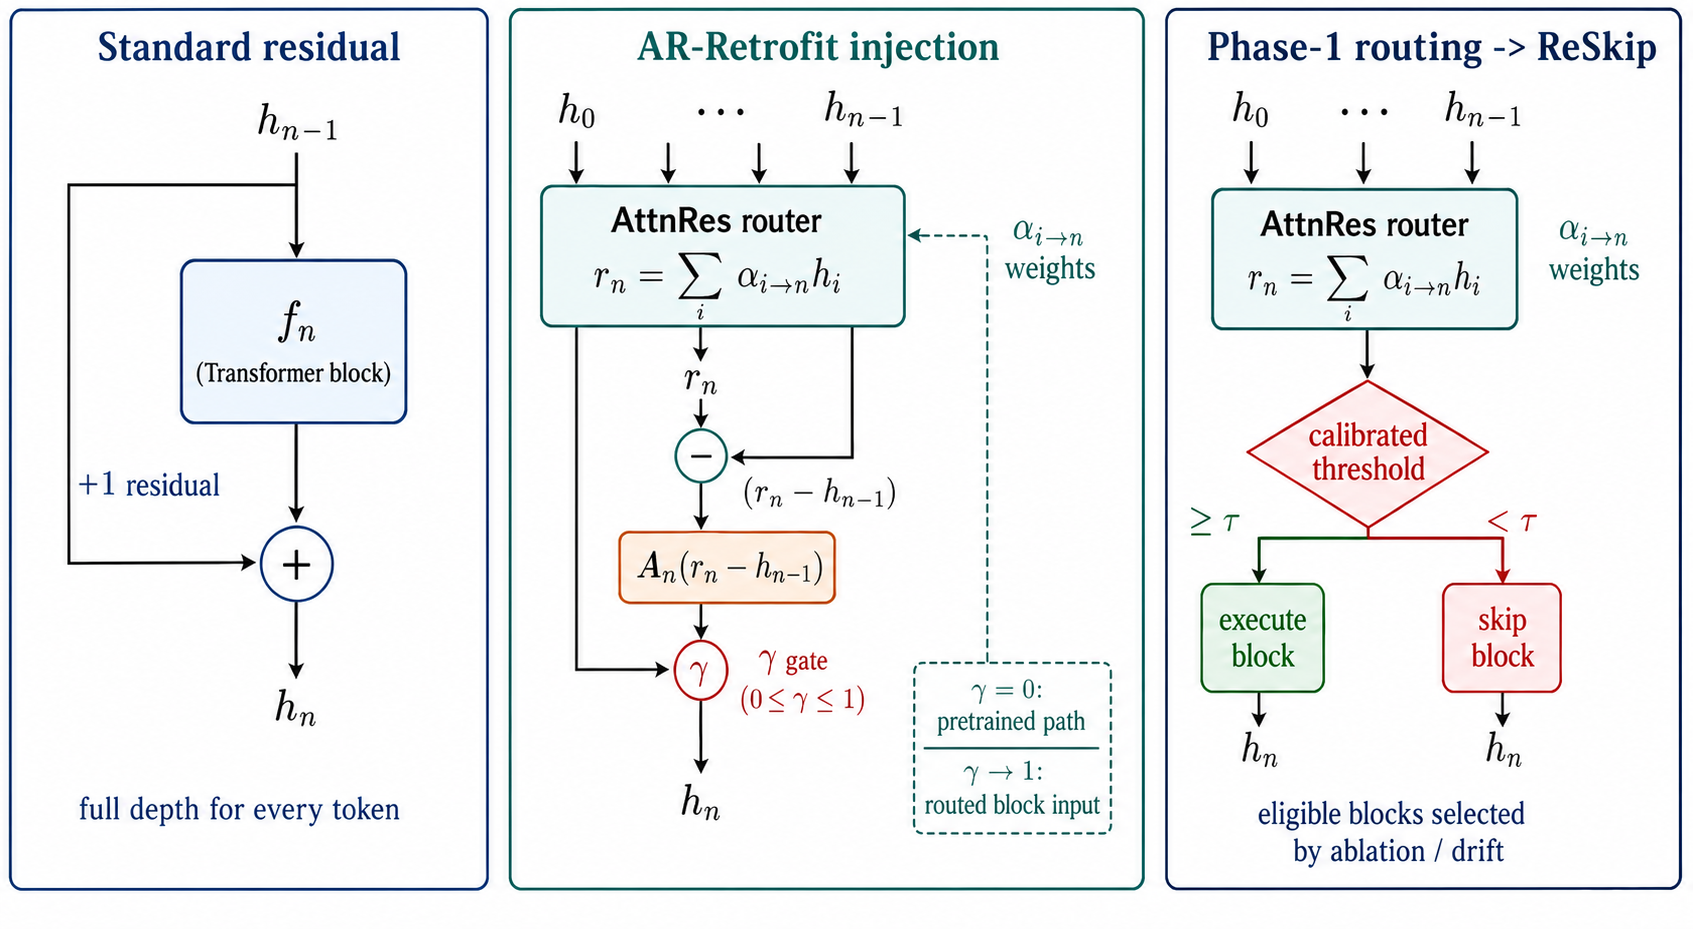
\includegraphics[width=\textwidth]{reskip_main_figure_v2.png}
\caption{\textbf{Overview of \reskip{} and \retrofit{}.}
Left: a standard transformer residual gives no intrinsic routing signal. Middle: \retrofit{} injects an identity-preserving $\gamma$-gated \attnres{} path into the frozen pretrained backbone. Right: the phase-1 \attnres{} weights are computed before block execution and are calibrated into \reskip{} decisions.}
\label{fig:overview}
\end{figure}


%----------------------------------------------------------------------
\section{Method}
\label{sec:method}
%----------------------------------------------------------------------

\subsection{Attention Residuals as a pre-execution routing signal}
\label{sec:background}

A standard transformer uses fixed scalar-$1$ combination, $\mathbf{x}_l = \mathbf{x}_{l-1} + f_l(\mathbf{x}_{l-1})$, emitting no routing signal. \attnres{}~\citep{chen2026attnres} replaces this with a learned attention over depth. Each block $l$ maintains a pseudo-query $\mathbf{w}_l \in \R^d$; keys are projections $\mathbf{k}_i = W_K \mathbf{h}_i$ of earlier block outputs $\mathbf{h}_i$, and
\begin{equation}
  \alpha_{i \to l} = \frac{\exp(\mathbf{w}_l^\top \mathbf{k}_i / \sqrt{d})}{\sum_{j=0}^{l-1} \exp(\mathbf{w}_l^\top \mathbf{k}_j / \sqrt{d})},
  \qquad
  \mathbf{x}_l = \sum_{i=0}^{l-1} \alpha_{i \to l}\,\mathbf{h}_i .
  \label{eq:attnres}
\end{equation}
The key property is two-phase execution. Computing the input to block $l$ requires only $\{\mathbf{h}_i\}_{i<l}$ and $\mathbf{w}_l$---both available \emph{before} $f_l$ runs. We call the pre-execution attention computation \emph{phase~1} and $f_l$ itself \emph{phase~2}. Phase~1 is the routing signal we exploit. Block-\attnres{} groups layers into $N$ blocks and applies the softmax at the block level, which is the granularity used throughout. Algorithm~\ref{alg:two_phase} gives the full two-phase forward with \reskip{}'s skip check folded in.

\subsection{\retrofit{}: installing the routing path}
\label{sec:retrofit}

The retrofit target is constrained by the problem in the introduction: take a transformer pretrained in the standard-residual regime and produce an \attnres{}-capable model that (P1) preserves benchmark quality, (P2) emits a routing $\alpha$ informative enough to drive \reskip{}, and (P3) trains in a single short fine-tune over off-the-shelf SFT data, with the base frozen. To satisfy the first constraint, the modification must be exactly identity-preserving at step $0$; to satisfy the second, the routing must feed the real forward path, not merely observe it.

We organise the decoder into $N$ \emph{blocks} of adjacent layers (Qwen3-VL-2B uses $7$ blocks of $4$ layers in the main experiments). For every block $n\ge 1$ we add an \attnres{} router $\mathbf{w}_n$, a tiny adapter $A_n$ (down-up bottleneck of rank $r$, SiLU), and a scalar gate $\gamma_n$:
\begin{equation}
  r_n = \sum_{i=0}^{n-1} \alpha_{i \to n}\,h_i, \qquad
  x_n = h_{n-1} + \gamma_n\,A_n(r_n - h_{n-1}), \qquad
  h_n = \mathrm{Block}_n(x_n).
  \label{eq:gamma_gate}
\end{equation}
$\mathrm{Block}_n$ is the pretrained block group, verbatim; \attnres{} enters \emph{between} blocks, as a correction. The retrofit parameters $\{\mathbf{w}_n, \gamma_n, A_n\}$ amount to $\sim$$7.4$M ($<0.4\%$) on 2B and $\sim$$11.8$M ($<0.3\%$) on 4B at the canonical $r{=}256$, $L{=}4$ partition; the entire base---embeddings, vision tower, decoder layers, LM head---is frozen.

With $\gamma_n{=}0$ we have $x_n = h_{n-1}$ exactly, so the forward at step $0$ is bit-identical to the pretrained model. The adapter up-projection is small-random ($\mathcal{N}(0,0.02^2)$) so that $\partial\mathcal{L}/\partial\gamma_n \ne 0$ at init, avoiding gradient deadlock. We then ramp $\gamma_n$ via a linear curriculum $0\to 1$ over the first $30$--$50\%$ of training. At $\gamma_n{=}1$, the \attnres{}-routed correction is fully active, but the model remains a residual correction on the pretrained stream as defined in Eq.~\ref{eq:gamma_gate}. Appendix~\ref{app:route_ablations} compares observer-only, interpolation, and informed-initialisation controls.

The training objective follows from the three constraints above. We minimise
\begin{equation}
  \mathcal{L} = \mathcal{L}_{\text{CE}}(\text{full path}) + \lambda_{\text{kl}}\,\mathcal{L}_{\text{KL}}(\text{skip path}\,\|\,\text{teacher}) + \lambda_{\text{ent}}\,\mathcal{L}_{\text{ent}}(\alpha) ,
  \label{eq:retrofit_loss}
\end{equation}
where the full-path CE is computed on assistant tokens, while the skip-branch KL samples one block at random per step, runs the forward with it skipped, and pulls the resulting logits toward a frozen pretrained teacher. This makes the surrogate $x_n$ useful both when the block runs and when it is skipped. $\mathcal{L}_{\text{ent}}$ is implemented with a negative sign in the loss, i.e., a light entropy-maximising prior against premature collapse of $\alpha$. Default $\lambda_{\text{kl}}{=}1$, entropy weight $0.02$, lr $10^{-3}$ on retrofit params, cosine schedule with $100$-step warmup. Hyperparameters and data mixtures are listed in Appendix~\ref{app:retrofit_hparams}.

This is not ordinary SFT. The CE term keeps the full path useful for the downstream task, but by itself it does not train the skipped surrogate to replace a real block. The skip-branch KL supplies that constraint by tying one skipped-block forward per step to the frozen teacher. Conversely, teacher imitation alone would merely reproduce the base model. The weak entropy prior prevents early one-source collapse while still allowing the router to sharpen later. This three-term structure is what makes the retrofit identity-preserving at step $0$, task-improving after training, and skip-ready at inference.

\subsection{\reskip{}: dynamic block skipping from the installed signal}
\label{sec:reskip}

\reskip{} uses the installed routing path rather than a separate controller. For block $n$, phase~1 computes $\alpha_{\cdot\to n}$ before the block body runs. We then read the weight $w_{\text{recent}}(n)$ that the router assigns to the immediate predecessor and decide whether to execute phase~2:
\begin{equation}
  \text{skip block $n$} \iff
  w_{\text{recent}}(n) > \tau_n
  \;\text{and}\;
  n \in \mathcal{P}
  \;\text{and}\;
  \textstyle\sum_{m<n} \mathbb{1}[\text{skipped}_m] < M_{\max} .
  \label{eq:skip_rule}
\end{equation}
The decision is available before the current block executes, so a trigger can actually save that block. When the rule fires, we short-circuit the block as $h_n\!\leftarrow\!x_n$, where $x_n$ is the routed-correction input in Eq.~\ref{eq:gamma_gate}. To keep autoregressive decoding cache-consistent, a skipped decoder layer still runs the K/V-producing slice ($\texttt{LayerNorm}\!\to\!\texttt{k/v\_proj}\!\to\!\texttt{RoPE}\!\to\!\texttt{cache.update}$) and skips \texttt{q\_proj}, attention, \texttt{o\_proj}, and MLP. The cache-enabled skip path matches the cacheless path in last-position argmax (Appendix~\ref{app:kv_equiv}).

\subsection{Calibration and safety selection}
\label{sec:calibration}

Routing weight is a usable depth signal, not a certificate that a block can be removed. Each eligible set $\mathcal{P}$ is therefore selected offline from two complementary diagnostics. The \attnres{} importance score
\[
I(n)=\max_{l>n}\,\E[\alpha_{n\to l}]
\]
measures how often future blocks refer to block $n$, while an ablation or drift score measures how costly it is to remove that block on the relevant distribution. For language experiments we use $A(n)=\mathrm{PPL}(\text{$n$ removed})/\mathrm{PPL}(\text{full})$; for VLA we use action-drift MSE on simulated rollouts. Thresholds $\tau_n$ are the $q$-th empirical quantile of $w_{\text{recent}}(n)$ on held-out calibration data. This separation is central: $\alpha$ decides \emph{when} a calibrated block looks locally redundant, while ablation or drift decides \emph{which} blocks are eligible to skip.

%----------------------------------------------------------------------
\section{Controlled Motivation: AttnRes and ReSkip at 340M}
\label{sec:controlled_340m}
%----------------------------------------------------------------------

\subsection{AttnRes and ReSkip at 340M}
\label{sec:exp_signal}

We first test the mechanism in the setting where \attnres{} is trained from scratch, before introducing any retrofit confound. On a 340M block-\attnres{} transformer ($d{=}1024$, $L{=}24$, $N{=}8$ blocks; FineWeb-Edu 100BT~\citep{penedo2024fineweb}; \texttt{lm-eval-harness}~\citep{eval-harness}), \reskip{} at $\mathcal{P}{=}\{3,5\}, M_{\max}{=}2, q{=}0.85$ matches the full-depth \attnres{} scores across the expanded language benchmark set and gives $1.19\times$ wall-clock at sequence length $8192$ (Tab.~\ref{tab:reskip_benchmark}; Pareto curves in Appendix~\ref{app:reskip_results}). The observed skip count averages $0.88$ blocks and varies $0$--$2$ per forward, confirming input-dependent allocation rather than a threshold that never fires.

\begin{figure}[t]
\centering
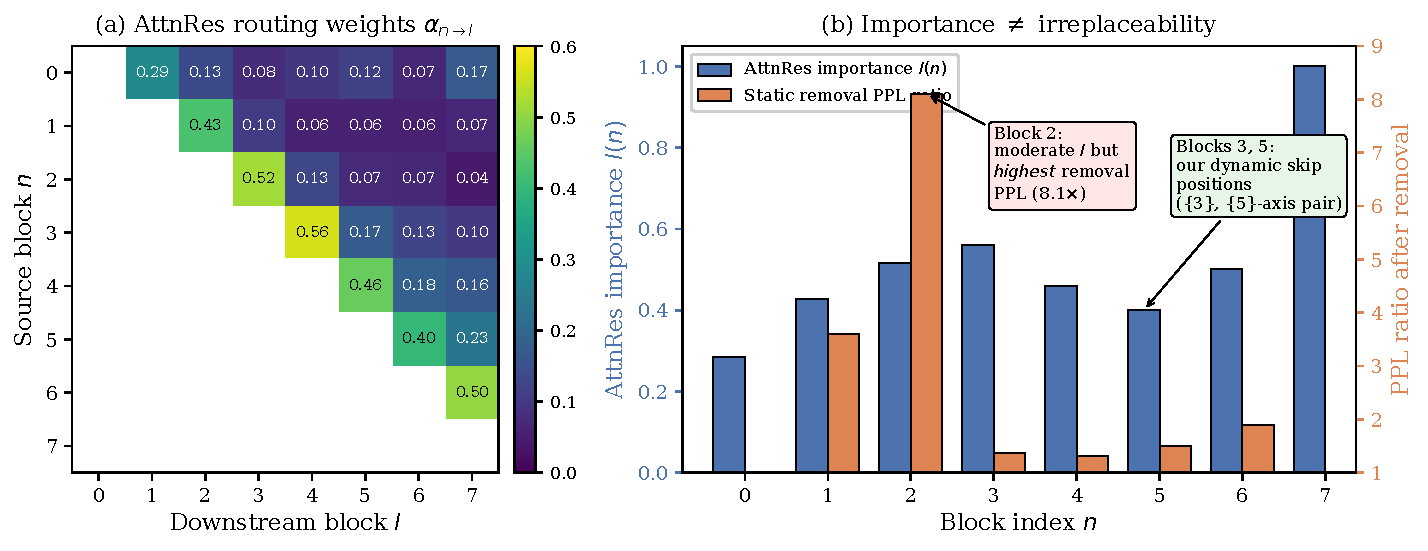
\includegraphics[width=0.95\textwidth]{reskip_routing_importance_vs_ablation.pdf}
\caption{\textbf{\attnres{} routing weights do not predict ablation impact (340M).} (a)~Learned block-level $\alpha_{n \to l}$. (b)~$I(n)$ (blue, left axis) and $A(n)$ (orange, right axis). \reskip{} uses routing for input-dependent decisions, but eligible blocks still need ablation-based safety selection.}
\label{fig:reskip_routing}
\end{figure}

\begin{table}[t]
\caption{\textbf{\reskip{} on 340M from-scratch \attnres{}.} The selected operating point preserves the full-depth \attnres{} scores on the expanded task set while actually firing: ReSkip averages $0.88$ skipped blocks over $48$ sequence-$8192$ batches and gives $1.19\times$ wall-clock at that length. Headline: \texttt{acc\_norm} for PIQA/HellaSwag/ARC-E/ARC-C/OpenBookQA, plain \texttt{acc} for MMLU/LAMBADA.}
\label{tab:reskip_benchmark}
\centering\small
\setlength{\tabcolsep}{3.5pt}
\resizebox{\textwidth}{!}{%
\begin{tabular}{lcccccccccc}
\toprule
Configuration & Avg.\ skip & Speed & LAMBADA acc & LAMBADA ppl & HellaSwag & PIQA & ARC-E & ARC-C & MMLU & OpenBookQA \\
\midrule
Vanilla (no \attnres{})                    & -- & -- & 0.3790 & 24.71 & 0.4436 & 0.6779 & \textbf{0.5602} & \textbf{0.3046} & \textbf{0.2594} & 0.3320 \\
\midrule
\attnres{} full-depth                       & $0.00$ & $1.00\times$ & 0.4054 & 20.20 & 0.4607 & 0.6893 & 0.5438 & 0.3012 & 0.2555 & 0.3580 \\
$+$ \reskip{} ($\{3,5\}, M{=}2, q{=}0.85$)  & $\mathbf{0.88}$ & $\mathbf{1.19\times}$ & \textbf{0.4054} & \textbf{20.20} & \textbf{0.4607} & \textbf{0.6893} & \textbf{0.5438} & \textbf{0.3012} & \textbf{0.2555} & \textbf{0.3580} \\
\bottomrule
\end{tabular}
}
\end{table}

This controlled study establishes the motivation for the retrofit experiments: \attnres{} improves the vanilla residual baseline, exposes a pre-execution depth signal, and lets \reskip{} recover wall-clock speed without changing the trained weights. We return to matched-rate and calibration ablations in Section~\ref{sec:ablations_main}.

%----------------------------------------------------------------------
\section{Retrofitting Qwen3-VL: VLM Quality, Runtime, and ReSkip}
\label{sec:experiments}
\label{sec:exp_retrofit}
%----------------------------------------------------------------------

\subsection{VLM adaptation: quality against the base}
\label{sec:exp_capability}

We retrofit \textbf{Qwen3-VL-2B}~\citep{bai2025qwen3vl} ($L{=}28, d{=}2048$) at $N{=}7$ blocks of $L{=}4$ and \textbf{Qwen3-VL-4B} ($L{=}36, d{=}2560$) at $N{=}9$ blocks of $L{=}4$. All base parameters are frozen; $\sim$$7.4$M ($2$B) / $\sim$$11.8$M ($4$B) retrofit parameters at $r{=}256$ train via Eq.~\ref{eq:retrofit_loss}. The final SFT mixture contains $60\%$ LLaVA-OneVision-Data~\citep{li2024llavaonevision}, $20\%$ UltraChat~\citep{ding2023ultrachat}, $10\%$ NuminaMath-CoT~\citep{aimo2024numinamath}, and $10\%$ OpenThoughts-114k~\citep{guha2025openthoughts} for $10$k steps; Appendix~\ref{app:data_mix} gives the concrete mixture. Evaluation uses LAMBADA~\citep{paperno2016lambada}/HellaSwag~\citep{zellers2019hellaswag} for text and six \texttt{lmms-eval} benchmarks for VLM (MMBench~\citep{liu2023mmbench}, MMMU~\citep{yue2024mmmu}, MMStar~\citep{chen2024mmstar}, AI2D~\citep{kembhavi2016ai2d}, OCRBench~\citep{liu2024ocrbench}, RealWorldQA~\citep{grok2024realworldqa}). Identity-at-init is verified before training ($\gamma{=}0$ reproduces base; max $|\Delta\text{logits}|=0.375$ bf16, $100\%$ argmax agreement; Appendix~\ref{app:identity}).

\begin{table}[t]
\caption{\textbf{\retrofit{} on Qwen3-VL-2B/4B at the canonical $L{=}4$ recipe} (\texttt{lmms-eval} full splits for VLM, $n{=}2000$ for LAMBADA/HellaSwag). The retrofit improves base on $5/6$ VLM benchmarks at both scales, with mean VLM gains of $+2.1$pp on $2$B and $+1.2$pp on $4$B, and lifts text on LAMBADA. MMStar overall holds; the math sub-category (Appendix~\ref{app:mmstar_subcat}) jumps $+7.9$pp on $2$B / $+3.9$pp on $4$B, consistent with a router that lifts deliberate-reasoning paths. Auxiliary parameter-matched LoRA controls do not show the same text-gain pattern (Appendix~\ref{app:lora_baselines}).}
\label{tab:retrofit_main}
\centering\small
\setlength{\tabcolsep}{4pt}
\begin{tabular}{lcccccccc}
\toprule
& \multicolumn{2}{c}{Text} & \multicolumn{6}{c}{VLM (\texttt{lmms-eval} full split)} \\
\cmidrule(lr){2-3}\cmidrule(lr){4-9}
Configuration & LAMBADA & HellaSwag & MMBench & MMMU & MMStar & AI2D & OCRBench & RWQA \\
\midrule
Qwen3-VL-2B (base)                    & 0.532 & 0.506 & 75.77 & 0.414 & 0.536 & 0.736 & 0.772 & 0.648 \\
$+$ \retrofit{} ($L{=}4$, $10$k)      & \textbf{0.5650} & 0.500   & \textbf{78.87} & \textbf{0.432} & 0.536 & \textbf{0.758} & \textbf{0.814} & \textbf{0.661} \\
~~~~$\Delta$ vs.\ base                & \textbf{+3.3}   & $-0.6$  & \textbf{+3.10} & \textbf{+1.8} & $0.0$  & \textbf{+2.2}  & \textbf{+4.2}  & \textbf{+1.3}  \\
\midrule
Qwen3-VL-4B (base)                    & 0.576 & 0.562 & 83.33 & 0.490 & 0.624 & 0.819 & 0.819 & 0.715 \\
$+$ \retrofit{} ($L{=}4$, $10$k)      & \textbf{0.6625} & 0.5515 & \textbf{85.22} & \textbf{0.521} & \textbf{0.632} & \textbf{0.825} & \textbf{0.824} & \textbf{0.718} \\
~~~~$\Delta$ vs.\ base                & \textbf{+8.7}   & $-1.1$ & \textbf{+1.9}  & \textbf{+3.1}  & \textbf{+0.8}  & \textbf{+0.6}  & \textbf{+0.5}  & \textbf{+0.3}  \\
\bottomrule
\end{tabular}
\end{table}


The retrofit improves base on five of six VLM benchmarks at both scales, averaging $+2.1$pp across the six VLM benchmarks on $2$B and $+1.2$pp on $4$B. The largest gain appears on the MMStar math subcategory ($+7.9$pp at $2$B, $+3.9$pp at $4$B; full $6$-cell decomposition in Appendix~\ref{app:mmstar_subcat}). The win concentrates on \emph{deliberate reasoning over images} rather than perception, consistent with a router that lifts deeper reasoning paths. Text quality also lifts: $+3.3$pp LAMBADA / $-16\%$ ppl on $2$B and $+8.7$pp / $-32\%$ on $4$B; HellaSwag is within $\pm 1.1$pp at both scales. Auxiliary parameter-matched LoRA controls on a related SFT mix do not recover the LAMBADA gain (Appendix~\ref{app:lora_baselines}). These controls do not prove that all quality gains come uniquely from routing, but they rule out a simple parameter-count-only explanation. We therefore treat the routed path as load-bearing for skip-ready behavior, while interpreting quality gains as consistent with, but not uniquely attributable to, the routed correction.

\subsection{Runtime and calibrated ReSkip after retrofit}
\label{sec:exp_reskip_tradeoff}

After \retrofit{} installs the routing path, \reskip{} can be applied without adding a separate router. On the canonical 2B retrofit, LAMBADA-$500$ at the conservative language operating point stays within $1.0$pp of the no-skip retrofit while skipping input-dependent blocks (Tab.~\ref{tab:retrofit_reskip_main}). The aggressive thresholds show the expected calibration boundary: once the threshold instructs the model to skip blocks it normally executes, quality drops sharply. Together with the runtime characterization in Tab.~\ref{tab:retrofit_latency}, this shows the target-scale behavior we want: the installed routing path preserves or improves model capability at near-base full-depth runtime, and \reskip{} turns that path into calibrated input-dependent depth allocation.

\begin{table}[t]
\caption{\textbf{Quality--skip behavior after retrofit.} LAMBADA-$500$ on the canonical $L{=}4$ 2B retrofit, $\mathcal{P}{=}\{1,4\}$, $M_{\max}{=}2$, with thresholds calibrated on $32$ held-out LAMBADA prefixes. The conservative point preserves quality while producing input-dependent block skipping; lower thresholds show the expected calibration boundary.}
\label{tab:retrofit_reskip_main}
\centering\small
\setlength{\tabcolsep}{4pt}
\begin{tabular}{lcccc}
\toprule
Configuration & LAMBADA acc & LAMBADA ppl & $\Delta$ acc vs no-skip & Avg.\ skipped blocks \\
\midrule
No-skip retrofit & $0.5700$ & $4.526$ & --- & $0.00$ \\
\retrofit{} $+$ \reskip{} ($q{=}0.85$) & $0.5600$ & $5.258$ & $-1.0$pp & $0.19$ \\
\retrofit{} $+$ \reskip{} ($q{=}0.50$) & $0.4120$ & $12.550$ & $-15.8$pp & $1.06$ \\
\retrofit{} $+$ \reskip{} ($q{=}0.30$) & $0.3900$ & $14.005$ & $-18.0$pp & $1.17$ \\
\bottomrule
\end{tabular}
\end{table}

The full-depth retrofit path remains close to the base when both models run under the same fixed-shape inference setting (Tab.~\ref{tab:retrofit_latency}). This is the practical runtime point: adding the routing path does not erase the quality gains with a large inference penalty, and the dynamic skip rule operates on top of that installed path.

\begin{table}[t]
\caption{\textbf{Full-depth runtime of the installed routing path.} Forward-pass latency on $1{\times}$H100, bf16, batch $1$, median of $20$ runs after $5$ warmup. The canonical compiled setting runs the retrofitted model within $2.9\%$ of the compiled base, while improving the quality metrics in Tab.~\ref{tab:retrofit_main}.}
\label{tab:retrofit_latency}
\centering\small
\setlength{\tabcolsep}{4pt}
\begin{tabular}{lccccc}
\toprule
Mode & seq & base (ms) & retrofit ($L{=}4$, ms) & retrofit / base & vs uncompiled base \\
\midrule
Uncompiled                                & $1024$ & $14.91$ & $16.66$ & $1.117\times$ & $1.117\times$ \\
Uncompiled                                & $2048$ & $25.49$ & $28.53$ & $1.119\times$ & $1.119\times$ \\
Compiled (\texttt{reduce-overhead})       & $2048$ & $21.31$ & $22.50$ & $1.056\times$ & $0.855\times$ \\
\textbf{Compiled (\texttt{max-autotune})} & $\mathbf{2048}$ & $\mathbf{21.81}$ & $\mathbf{22.43}$ & $\mathbf{1.029\times}$ & $\mathbf{0.864\times}$ \\
\bottomrule
\end{tabular}
\end{table}

The block partition and mixture choices are reported in the appendix rather than treated as the main story. $L{=}4$ sits on the accuracy plateau alongside nearby block sizes and reduces router calls; the final mixture is the one that preserves VLM capability while training the routed correction. Full block-partition, data-mixture, and design-control ablations are in Appendices~\ref{app:block_partition},\,\ref{app:data_mix},\,\ref{app:retrofit_ablation}.


%----------------------------------------------------------------------
\section{VLA Transfer Evidence}
\label{sec:vla}
%----------------------------------------------------------------------

A VLA test asks whether the retrofitted routed-depth signal remains usable beyond VLM evaluation. Vision tokens (perceptual, early-layer~\citep{raghu2021vision}), language tokens (task spec.), and action tokens (motor planning) have no principled reason to share effective depth; \attnres{} routing gives a per-position handle on this without token-level gating machinery.

We attach the OpenVLA-OFT~\citep{kim2025openvlaoft} action head ($L_1$ regression, no chunking) to Qwen3-VL-2B/4B backbones (ViT frozen) and train on the pooled \texttt{libero\_all} mix from LIBERO~\citep{liu2023libero}. The main comparison is deliberately narrow: \textbf{Path 0} uses the stock backbone with OFT, while \textbf{Path B} warm-starts from our canonical $L{=}4$ VLM retrofit and keeps $\gamma_n{=}1$ throughout. Both paths share the same action head, data, and $30$k-step OFT schedule on $4{\times}$H100 ZeRO-2 with effective batch $32$. Each policy is evaluated for $500$ rollouts per suite ($2{,}000$ per policy). The VLA in-backbone forward uses the same installed routing path as the VLM retrofit; at sequence length $2048$ its eager latency is $28.79$\,ms vs.\ $25.49$\,ms for the stock backbone, within $1\%$ of the VLM retrofit runtime (Appendix~\ref{app:latency}).

\subsection{LIBERO results}
\label{sec:vla_results}

\begin{table}[t]
\caption{\textbf{LIBERO 4-suite success rates (\%)} for Qwen3-VL-2B/4B. Entries are success rates over $500$ rollouts per suite ($2{,}000$ per policy). \emph{Path 0} is the stock-backbone OFT baseline; \emph{Path B} warm-starts from our $L{=}4$ VLM retrofit. The table is supporting transfer evidence for the retrofit pathway rather than a broad robotics claim.}
\label{tab:vla_libero}
\centering\small
\setlength{\tabcolsep}{4pt}
\begin{tabular}{llcccccc}
\toprule
Scale & Path (steps) & Spatial & Object & Goal & Long-$10$ & \textbf{Avg} & $\Delta$ vs.\ Path 0 \\
\midrule
2B & Path 0 ($30$k)                & $94.8$ & $99.8$ & $97.4$ & $91.4$ & $95.85$ & --- \\
2B & \textbf{Path B ($30$k, ours)} & $\mathbf{97.8}$ & $99.6$ & $\mathbf{98.6}$ & $\mathbf{92.6}$ & $\mathbf{97.15}$ & $\mathbf{+1.30}$ \\
\midrule
4B & Path 0 ($30$k)                & $95.0$ & $99.2$ & $97.8$ & $92.2$ & $96.05$ & --- \\
4B & \textbf{Path B ($30$k, ours)} & $94.6$ & $\mathbf{99.8}$ & $\mathbf{98.2}$ & $\mathbf{94.2}$ & $\mathbf{96.70}$ & $\mathbf{+0.65}$ \\
\bottomrule
\end{tabular}
\end{table}

Path B reaches $97.15\%$ on $2$B and $96.70\%$ on $4$B. The gain concentrates on Spatial ($+3.0$pp at $2$B) and Long-$10$ ($+2.0$pp at $4$B), where we observe the clearest gains in this evaluation. We use these results as downstream transfer evidence for \retrofit{}, not as a broad robotics claim. Appendix~\ref{app:vla_variance} reports repeated-rollout sensitivity.

\subsection{\reskip{} on the action stream: calibrated conservative skipping}
\label{sec:vla_reskip}

We now apply the same \reskip{} rule at inference on the trained Path B policies, with thresholds calibrated on a sim-rollout distribution rather than language tokens (the rationale is in the next paragraph). Eligible blocks are picked per scale from a per-block action-drift sweep (Appendix~\ref{app:vla_pareto}: $\mathcal{P}{=}\{1,4\}$ on $2$B, $\mathcal{P}{=}\{1,2\}$ on $4$B) and $M_{\max}{=}2$ throughout. Tab.~\ref{tab:vla_reskip_pareto} shows the $4$-suite Pareto across $q$.

\begin{table}[t]
\caption{\textbf{\reskip{} 4-suite Pareto} on the trained Path B policies. Eligible blocks $\mathcal{P}$ and threshold $\tau$ are calibrated per scale on the action distribution; $q$ is the empirical quantile that produces $\tau$. The conservative end ($q{=}0.99$) preserves success rates in this evaluation.}
\label{tab:vla_reskip_pareto}
\centering\small
\setlength{\tabcolsep}{4pt}
\begin{tabular}{lccccc}
\toprule
$q$ (sim-calibrated) & Spatial & Object & Goal & Long-$10$ & \textbf{Avg} \\
\midrule
\multicolumn{6}{l}{\emph{Qwen3-VL-2B, $\mathcal{P}{=}\{1,4\}, M{=}2$, no-skip/full ref $97.2$}} \\
\midrule
$0.30$              & $4.7$  & ---     & ---     & ---     & (sharp drop) \\
$0.85$              & $80.0$ & $98.0$  & $87.3^\ast$ & $67.2$  & $83.1$ \\
$0.95$              & $95.0$ & $99.4$  & $97.6$  & $86.8$  & $94.7$ \\
$\mathbf{0.99}$     & $\mathbf{97.6}$ & $\mathbf{99.2}$  & $\mathbf{99.0}$  & $\mathbf{93.6}$  & $\mathbf{97.4}$ \\
no-skip/full (ref)  & $97.8$ & $99.6$  & $98.6$  & $92.6$  & $97.2$ \\
\midrule
\multicolumn{6}{l}{\emph{Qwen3-VL-4B, $\mathcal{P}{=}\{1,2\}, M{=}2$, no-skip/full ref $96.7$}} \\
\midrule
$0.30$              & $89.6$ & $95.4$  & $96.4$  & $86.0$  & $91.85$ \\
$0.50$              & $91.2$ & $98.0$  & $98.2$  & $89.6$  & $94.25$ \\
$0.85$              & $93.6$ & $99.2$  & $97.6$  & $93.2$  & $95.90$ \\
$0.95$              & $95.6$ & $98.0$  & $98.0$  & $93.0$  & $96.15$ \\
$\mathbf{0.99}$     & $\mathbf{96.4}$ & $\mathbf{98.2}$  & $\mathbf{98.4}$  & $\mathbf{92.8}$  & $\mathbf{96.5}$ \\
no-skip/full (ref)  & $94.6$ & $99.8$  & $98.2$  & $94.2$  & $96.7$ \\
\bottomrule
\multicolumn{6}{p{14cm}}{\footnotesize $^\ast$Partial eval ($332/500$ trials) — driver schedule cut short; reported as the rate over completed trials.}
\end{tabular}
\end{table}

Thresholds are calibrated on the action distribution rather than transferred from language. The reason is that $q$ is not itself a skip rate; it indexes an empirical distribution of $w_{\text{recent}}$ that shifts across modalities. The recommended VLA point is therefore conservative ($q{=}0.99$): it skips rarely, but only on blocks whose action-drift sweep says they are locally safe.


%----------------------------------------------------------------------
\section{Ablations: Skip Budget and Calibration}
\label{sec:ablations_main}
%----------------------------------------------------------------------

The main knobs in \reskip{} are the eligible set $\mathcal{P}$, the skip budget $M_{\max}$, and the calibration quantile $q$. Table~\ref{tab:budget_calibration_main} summarizes the operating points used in the main experiments. The 340M result shows that increasing the budget from no-skip to $M_{\max}{=}2$ can produce a real speedup when the skip signal is native to the trained \attnres{} model. On the retrofitted VLM and VLA, the conservative $M_{\max}{=}2$ settings preserve quality while using the installed routing path characterised in Tables~\ref{tab:retrofit_latency} and~\ref{tab:vla_reskip_pareto}.

\begin{table}[t]
\caption{\textbf{Skip-budget and calibration operating points.} Quality is reported in the native metric for each setting. Runtime is measured directly for the 340M controlled model and for full-depth Qwen3-VL retrofit; the retrofitted \reskip{} rows report the corresponding average skipped blocks or success-rate Pareto point.}
\label{tab:budget_calibration_main}
\centering\small
\setlength{\tabcolsep}{4pt}
\begin{tabular}{llcccc}
\toprule
Setting & Configuration & $M_{\max}$ & $q$ & Quality & Depth / runtime behavior \\
\midrule
340M \attnres{} & full-depth & $0$ & -- & LAMBADA $0.4054$ / ppl $20.20$ & $1.00\times$, $0.00$ skips \\
340M \attnres{} & \reskip{} & $2$ & $0.85$ & LAMBADA $0.4054$ / ppl $20.20$ & $1.19\times$, $0.88$ avg skips \\
2B VLM retrofit & full-depth & $0$ & -- & LAMBADA $0.5700$ / ppl $4.526$ & $22.43$ ms compiled \\
2B VLM retrofit & \reskip{} & $2$ & $0.85$ & LAMBADA $0.5600$ / ppl $5.258$ & $0.19$ avg skips \\
2B VLA Path B & \reskip{} & $2$ & $0.99$ & LIBERO avg $97.4\%$ & conservative action-stream skipping \\
4B VLA Path B & \reskip{} & $2$ & $0.99$ & LIBERO avg $96.5\%$ & conservative action-stream skipping \\
\bottomrule
\end{tabular}
\end{table}

The routing signal matters beyond the choice of skip locations. At a matched skip budget on the same 340M model, an input-dependent rule based on phase-1 routing preserves substantially more quality than static or random schedules (Tab.~\ref{tab:decision_main}). The dynamic rule is not always lossless at this more aggressive calibration point, but it is clearly better than skipping the same positions unconditionally.

\begin{table}[t]
\caption{\textbf{Dynamic, static, and random skip rules at matched rate on 340M.} All rows use the same trained \attnres{} weights, $\mathcal{P}{=}\{3,5\}$, and $M_{\max}{=}1$. Dynamic \reskip{} uses a calibrated phase-1 statistic; static and random controls remove the same positions without input dependence. Full decision-rule ablation and observed trigger rates are in Appendix~\ref{app:b1b2_decision_rule}.}
\label{tab:decision_main}
\centering\small
\setlength{\tabcolsep}{5pt}
\begin{tabular}{lccccc}
\toprule
Rule & LAMBADA & HellaSwag & PIQA & ARC-E & OpenBookQA \\
\midrule
Full-depth \attnres{} & $0.4054$ & $0.4607$ & $0.6893$ & $0.5438$ & $0.3580$ \\
\textbf{Dynamic \reskip{}} & $\mathbf{0.3445}$ & $\mathbf{0.4471}$ & $\mathbf{0.6774}$ & $\mathbf{0.5391}$ & $\mathbf{0.3540}$ \\
Static skip $P{=}3$ & $0.2624$ & $0.3968$ & $0.6610$ & $0.5206$ & $0.3300$ \\
Static skip $P{=}5$ & $0.2189$ & $0.4223$ & $0.6638$ & $0.5253$ & $0.3260$ \\
Random $\{P{=}3$ or $P{=}5\}$ & $0.2416$ & $0.4028$ & $0.6420$ & $0.5101$ & $0.3300$ \\
\bottomrule
\end{tabular}
\end{table}



%----------------------------------------------------------------------
\section{Related Work}
\label{sec:related}
%----------------------------------------------------------------------

For test-time compute, o1~\citep{openai2024o1}, DeepSeek-R1~\citep{deepseek2025r1}, chain-of-thought~\citep{wei2022chain}, and optimal test-time compute analyses~\citep{snell2024scaling} allocate compute by emitting more reasoning \emph{tokens}; per-token depth remains fixed. Depth-axis methods include ACT / Universal Transformers~\citep{graves2016adaptive, dehghani2018universal}, CALM~\citep{schuster2022confident}, Mixture-of-Depths~\citep{raposo2024mixture}, LayerSkip~\citep{elhoushi2024layerskip}, and static pruning~\citep{gromov2024unreasonable, men2024shortgpt}. These add a halting head, exit classifier, router, speculative decoder, or static removal rule. We instead use \attnres{} as an intrinsic routing signal produced by the forward pass itself, then retrofit that signal into an existing pretrained backbone. Appendix~\ref{app:b1b2_decision_rule} compares dynamic, static, and random skip rules at 340M, and Appendix~\ref{app:gromov_pruning} gives a full-layer static-pruning baseline at the VLM scale.

Table~\ref{tab:closest_methods} summarises the closest method-level distinction. The relevant distinction is the combination of frozen-backbone retrofitting and a pre-execution signal that is also part of the forward path.

\begin{table}[t]
\caption{\textbf{Closest method comparison.} The relevant distinction is the combination of frozen-backbone retrofitting and a pre-execution signal that is also part of the forward path.}
\label{tab:closest_methods}
\centering\small
\setlength{\tabcolsep}{3pt}
\resizebox{\textwidth}{!}{%
\begin{tabular}{lccccc}
\toprule
Method & Pretrained backbone & Extra decision head/router & Decision before current block & Applies to frozen pretrained backbone & Same signal forms input and skip \\
\midrule
Early exit / CALM & yes & yes & no & no & no \\
Mixture-of-Depths & train-time design & yes & yes & no & no \\
Static pruning & yes & no & yes & yes & no \\
LayerSkip & continued training & no / separate exit policy & partly / speculative & no & no \\
\attnres{} pretraining & no & no & yes & no & yes \\
\textbf{\retrofit{} $+$ \reskip{}} & \textbf{yes} & \textbf{no} & \textbf{yes} & \textbf{yes} & \textbf{yes} \\
\bottomrule
\end{tabular}
}
\end{table}

The neural motivation is recurrence as flexible effective depth. The dual-process distinction~\citep{kahneman2011thinking} maps naturally onto visual processing: easy stimuli can be handled by feedforward sweeps, while harder stimuli recruit recurrent circuits~\citep{lamme2000distinct, kar2019recurrent, dicarlo2012does}. Recurrent networks capture human representational dynamics~\citep{kietzmann2019recurrence}; \citet{spoerer2020recurrent} are the closest conceptual antecedent, showing that recurrent CNNs can spend more steps on harder images to explain speed--accuracy behaviour. Recurrence also has a depth interpretation: finite recurrence can be unrolled into feedforward depth, but the recurrent form reuses a fixed substrate for flexible effective depth~\citep{vanbergen2020going}. We take this as a design target, not a cognitive-faithfulness claim: cortical microcircuits and dendritic association~\citep{bastos2012canonical, buschman2007topdown, larkum2013cellular} motivate intrinsic routing, while our implementation is a transformer retrofit.

In residual architectures, DenseNet~\citep{huang2017densely} and Highway networks~\citep{srivastava2015highway} modify residual flow; \attnres{}~\citep{chen2026attnres} generalises residual combination with depth attention. To our knowledge, this is the first work to use \attnres{} weights as a pre-execution skip signal and to retrofit an \attnres{}-style routing path into pretrained transformers. In VLA, RT-2~\citep{brohan2023rt}, Octo~\citep{team2024octo}, OpenVLA~\citep{kim2024openvla}, and Pi0~\citep{black2024pi0} established the paradigm, while efficiency work has focused mainly on action chunking~\citep{zhao2023learning} and post-hoc compression. We contribute modality-aware adaptive depth for the VLM backbone.

\section{Discussion}
\label{sec:discussion}
%----------------------------------------------------------------------

\retrofit{} shows that a frozen pretrained transformer can acquire a pre-execution depth-routing path through a short identity-preserving fine-tune. \reskip{} shows that this installed signal can be calibrated into input-dependent block execution, with ablation or drift checks determining which blocks are safe to skip. The current evidence is strongest for the retrofit mechanism and calibrated dynamic-depth behavior; broader backbone coverage, stronger end-to-end acceleration, and per-modality token-level calibration remain open.

\bibliography{references}

%----------------------------------------------------------------------
\appendix
\section{Limitations and future work}
\label{app:limitations}
%----------------------------------------------------------------------

\paragraph{Limitations.}
(i)~Two retrofit targets from one VLM family; extension to InternVL / Gemma-VL / text-only LMs is planned. (ii)~Runtime measurements are H100 / bf16 / batch $1$ and use standard PyTorch inference paths; lower-end GPU / edge measurement is not yet done. (iii)~The current \reskip{} rule is block-level, inherited from \attnres{}; per-token routing and fused production kernels are future work. (iv)~The VLA Pareto thresholds are sim-calibrated per scale, not per modality \emph{within} a single rollout; per-modality, per-token-class calibration is the next sweep.

\paragraph{Future work: weight-shared AttnRes (\reloop{}).}
A natural extension shares block weights across depth and differentiates each application via position-indexed pseudo-queries; the \attnres{} routing statistic can then serve both \reskip{}'s high-immediate-predecessor skip rule and a \reloop{} halt rule based on low marginal change across recurrent applications. A 74M validation produced a smooth depth--quality Pareto ($25\%$ compute saved at $<1\%$ ppl change); scaling and combining with the retrofit framework is open.

\section{Implementation details}
\label{app:implementation}
%----------------------------------------------------------------------

\subsection{Online softmax merge with skip}
When a block is skipped, the online softmax merge simply does not process its output. The running state $(\mathbf{s}, m, e)$ is unchanged. The output is mathematically equivalent to an \attnres{} model trained without that block contributing---modulo the calibration of downstream $\mathbf{w}_l$.

\subsection{Pseudo-query initialisation (Section~\ref{sec:reskip} from-scratch)}
For from-scratch training we use $\mathbf{w}_l \sim \mathcal{N}(0, 0.02)$, yielding near-uniform $\alpha$ at initialisation that specialises over the first few thousand steps.

\subsection{Retrofit hyperparameters}
\label{app:retrofit_hparams}
AdamW with $\beta{=}(0.9,0.95)$, weight decay~$0$, gradient clip~$1.0$, bfloat16. Learning rate $10^{-3}$ for retrofit params (routers, adapters, $\gamma$), cosine schedule with $100$-step warmup. Sequence length~$1536$ (training), $2048$ (evaluation). Loss weights $\lambda_{\text{kl}}{=}1$, entropy weight $0.02$, KD temperature~$1$. The entropy term is subtracted from the loss, so it maximises routing entropy early in training rather than minimising it. Skip-branch sampling: one eligible block chosen uniformly at random per step. Adapter bottleneck rank $r{=}256$ (canonical); position-bias on router keys enabled; router temperature fixed at~$1$. $\gamma$-curriculum: $0\to 1$ linearly over the first $30\%$ of total steps (2B $5$k/$10$k, 4B $5$k), with ramp-fraction $0.5$ on 4B $\times 10$k to stabilise a late-stage $\gamma{=}1$ transition divergence (Appendix~\ref{app:gamma_stability}). Total training wall-clock on a single H100: $\sim$$22$ min for 2B $5$k, $\sim$$44$ min for 2B $10$k, $\sim$$54$ min for 4B $10$k.

\subsection{Block granularity}
\label{app:block_granularity}
For the final recipe we use $L{=}4$ layers per block on both scales: Qwen3-VL-2B has $N{=}7$ blocks and Qwen3-VL-4B has $N{=}9$ blocks. Earlier $L{=}2$ runs remain in the appendix as ablation controls, but $L{=}4$ is the canonical setting because it preserves the accuracy plateau while halving router calls relative to $L{=}2$. Each block receives one router, one residual adapter ($r{=}256$ default), and a scalar $\gamma$ gate.

\subsection{Identity-at-init details}
\label{app:identity}
With $\gamma_n{=}0$ and the adapter up-projection initialised at $\mathcal{N}(0, 0.02^2)$, the retrofit forward is arithmetically identical to the pretrained model (both produce $x_n = h_{n-1}$, which is passed into the unmodified block). We verified end-to-end: at $n{=}500$ on LAMBADA the retrofit and the base agree to within bfloat16 evaluation noise (acc $0.530$ vs.\ $0.532$; ppl $5.572$ vs.\ $5.547$); on MMMU and MMStar they are bit-equal at the answer-choice level. The smoke test at the token level shows max $|\Delta\text{logits}| = 0.375$ (bfloat16 SDPA noise) and $100\%$ argmax agreement on our calibration prompts.

\subsection{\texorpdfstring{Skip under \texttt{use\_cache=True}: correctness verification}{Skip under use cache: correctness verification}}
\label{app:kv_equiv}
We verify that the K/V-only skip path described in \S\ref{sec:retrofit} produces an argmax-consistent output with the cacheless path. Procedure: for a fixed prefill input, run the retrofit twice with the same skip configuration---once with \texttt{use\_cache=False} and once with \texttt{use\_cache=True}---and compare the last-position argmax and the logits. We swept skip sets $\{[4]$, $[4,10]$, $[4,10,12]$, $[2,4,10]\}$ on H\_r256\_5k on Qwen3-VL-2B. In every configuration the last-position argmax matches between the two cache regimes, and the maximum logit delta is $0.19$--$0.37$, identical to the bfloat16 SDPA jitter observed on the stock base with no retrofit and no skip. Multi-step autoregressive divergence starting around position $27$--$40$ is an inherent property of HF $+$ bf16 $+$ SDPA that the stock base exhibits on the same prompts (measured on ``Once upon a time'' and ``def fibonacci''); it is not a property of our skip path.

\subsection{\texorpdfstring{$\gamma{=}1$ transition stability}{gamma=1 transition stability}}
\label{app:gamma_stability}
The $\gamma$ curriculum is used to keep the frozen residual stream close to its pretrained operating point while the routed correction becomes active. Across the reported $2$B and $4$B canonical runs, we use a ramp that reaches $\gamma{=}1$ after at least $5{,}000$ optimisation steps. This schedule was stable across the scales and block partitions reported in the paper and does not confound the quality comparisons in Appendix~\ref{app:block_partition}.

%----------------------------------------------------------------------
\section{Retrofit ablations and inference machinery}
\label{app:ablations}
%----------------------------------------------------------------------

\subsection{Design controls}
\label{app:route_ablations}
We compared the $\gamma$-gated residual injection against three simpler designs: observer-only routing, block-input interpolation, and direct \attnres{} replacement with informed pseudo-query initialisation. These controls either made the routing weights non-load-bearing, moved the frozen backbone too abruptly away from its pretrained residual stream, or required substantially more tuning than the short retrofit budget. The $\gamma$-gated injection of \S\ref{sec:retrofit} is the stable recipe used in all main experiments.

\subsection{Adapter-rank ablation}
\label{app:rank_ablation}
Wall-clock latency is essentially unchanged across ranks ($\pm 2\%$ at all measured sequence lengths): the adapter's $2048{\to}r{\to}2048$ bottleneck is a small contributor compared to the router stack/softmax/einsum cost. Rank therefore affects quality but not speed. The canonical $r{=}256$ was selected from the $\gamma{\to}1$ ablation of Appendix~\ref{app:retrofit_ablation}; at equal step budgets lower ranks leave more of the MMBench drop on the table without compensating latency savings.

\subsection{\texorpdfstring{$\gamma{\to}1$ retrofit ablation}{gamma-to-1 retrofit ablation}}
\label{app:retrofit_ablation}
We swept variants of the canonical $\gamma{\to}1$ recipe along four axes: adapter rank $r\in\{32,64,128,256\}$, training steps $\in\{5\text{k},10\text{k},20\text{k}\}$, LLaVA-Instruct fraction of the mix $\in\{50\%,80\%\}$, and $\gamma$ ramp-fraction $\in\{0.3,0.7\}$. All other hyperparameters (loss, optimizer, schedule family, seed) are held constant.

\begin{table}[h]
\caption{\textbf{Retrofit ablation} on Qwen3-VL-2B. All rows use the $\gamma$-curriculum $0{\to}1$ over the first $30\%$ of steps unless noted. ``n=300 MMBench noise floor $\pm 1$ question'' corresponds to $\pm 0.33$pp.}
\label{tab:retrofit_ablation}
\centering\small
\begin{tabular}{lcccccrrr}
\toprule
Name & $\gamma$ sched & rank & steps & VLM\% & ramp & LAMBADA & HellaSwag & MMBench \\
\midrule
Base Qwen3-VL-2B & --- & --- & --- & --- & --- & $0.532$ & $0.506$ & $0.727$ \\
\midrule
\textbf{Canonical} & $0{\to}1$ fast & $\mathbf{256}$ & $\mathbf{5}$k & $\mathbf{50}$ & $\mathbf{0.3}$ & $\mathbf{0.576}$ & $\mathbf{0.522}$ & $\mathbf{0.710}$ \\
$+$ low rank      & $0{\to}1$ fast & $64$  & $10$k & $50$ & $0.3$ & $0.570$ & $0.530$ & $0.697$ \\
$+$ very low rank & $0{\to}1$ fast & $32$  & $10$k & $50$ & $0.3$ & $0.568$ & $0.526$ & $0.683$ \\
$+$ low rank, VLM-heavy & $0{\to}1$ fast & $64$  & $10$k & $80$ & $0.3$ & $0.560$ & $0.524$ & $0.660$ \\
$+$ mid rank, VLM-heavy & $0{\to}1$ fast & $128$ & $10$k & $80$ & $0.3$ & $0.564$ & $0.520$ & $0.653$ \\
$+$ VLM-heavy     & $0{\to}1$ fast & $256$ & $10$k & $80$ & $0.3$ & $0.560$ & $0.520$ & $0.617$ \\
$+$ longer, $10$k & $0{\to}1$ fast & $256$ & $10$k & $50$ & $0.3$ & $0.586$ & ---     & $0.587$ \\
$+$ slow ramp     & $0{\to}1$ slow & $256$ & $10$k & $50$ & $0.7$ & $0.568$ & $0.520$ & $0.517$ \\
$+$ longer, $20$k & $0{\to}1$ fast & $256$ & $20$k & $50$ & $0.3$ & $0.568$ & $0.520$ & $0.513$ \\
\bottomrule
\end{tabular}
\end{table}

\paragraph{Over-training signature at $\gamma{=}1$.} Holding ($r{=}256$, $50\%$ VLM, fast ramp) fixed and varying only the total step count, MMBench is strictly monotonic in steps: $5$k $\to 0.710$ (preserved), $10$k $\to 0.587$ ($-$14pp), $20$k $\to 0.513$ ($-$21pp). LAMBADA peaks at $10$k ($0.586$) and regresses at $20$k ($0.568$), so longer training buys no text-domain gain either. The $\gamma{=}1$ regime has a narrow compute sweet spot; past it the router+adapter over-specialise to the training distribution and the frozen backbone, unable to adapt further, loses its multimodal calibration.

\paragraph{Rank and data are subordinate.} Halving rank at $10$k recovers some MMBench ($r{=}32$: $0.683$, $r{=}64$: $0.697$), but never reaches the $5$k-$r{=}256$ level ($0.710$). Pushing the mix to $80\%$ LLaVA \emph{worsens} MMBench at every rank, indicating the regression is router over-adaptation to \emph{any} narrow training distribution, not insufficient visual exposure.

\paragraph{Interpretation.} These ablations are used only to set the canonical recipe. They are not the main evidence for \reskip{}; the load-bearing evidence is that the installed routing path participates in the forward computation and supports the calibrated skip rule in \S\ref{sec:exp_reskip_tradeoff}.

\subsection{Per-block skip importance}
\label{app:block_removal}
Running single-block removals on the canonical 2B retrofit gives the eligibility set used in the main text, $\mathcal{P}{=}\{1,4\}$ (Tab.~\ref{tab:retrofit_reskip_main}). The same qualitative ranking pattern appears across the 340M from-scratch and 2B retrofit settings: some blocks near the embedding or late residual-refinement stages are costly to remove, while selected mid-depth positions are safer candidates after per-model calibration.

\subsection{Calibration set (dynamic skip)}
\label{app:calibration}
Calibration uses 32 held-out LAMBADA prefixes (truncated to 512 tokens each). Per-block $w_{\text{recent}}(n)$ samples are collected with a single retrofit forward and the empirical quantile at $q$ is used as $\tau_n$. We verified that varying the calibration draw shifts $\tau_n$ by $<0.01$ in absolute terms at the chosen $q{=}0.95$. For VLA deployment, the identical calibration pipeline applied to the VLA in-backbone forward (\texttt{retrofit/eval/calibrate\_vla\_thresholds.py}) produces thresholds byte-identical to the LAMBADA-calibrated set on matched inputs, confirming that the VLA and VLM forwards instantiate the same router.

\subsection{Canonical data mixture}
\label{app:data_mix}

Table~\ref{tab:data_mix_ablation} gives the final SFT mixture used for the canonical retrofit. The mix is intentionally VLM-anchored, with a smaller math/reasoning component to strengthen deliberate reasoning without moving the frozen VLM backbone away from visual instruction following.

\begin{table}[h]
\caption{\textbf{Canonical retrofit SFT mixture.} The same source proportions are used for the $2$B and $4$B canonical $L{=}4$ recipes in Tab.~\ref{tab:retrofit_main}.}
\label{tab:data_mix_ablation}
\centering\small
\setlength{\tabcolsep}{6pt}
\begin{tabular}{lcl}
\toprule
Source & Proportion & Role \\
\midrule
LLaVA-OneVision-Data~\citep{li2024llavaonevision} & $60\%$ & visual instruction anchor \\
UltraChat~\citep{ding2023ultrachat} & $20\%$ & general instruction following \\
NuminaMath-CoT~\citep{aimo2024numinamath} & $10\%$ & mathematical reasoning traces \\
OpenThoughts-114k~\citep{guha2025openthoughts} & $10\%$ & open-ended reasoning traces \\
\bottomrule
\end{tabular}
\end{table}

This mixture is the only data recipe used for the canonical results in the main paper.

\subsection{Two-phase forward with dynamic skip (algorithm)}
\label{app:algorithm}
\begin{algorithm}[h]
\caption{Two-phase \attnres{} forward with dynamic \reskip{}.}
\label{alg:two_phase}
\begin{algorithmic}[1]
\STATE \textbf{Input:} embeddings $\mathbf{h}_0$; block functions $f_1,\dots,f_N$; pseudo-queries $\{\mathbf{w}_n\}$; eligible $\mathcal{P}$; thresholds $\{\tau_n\}$; max skips $M_{\max}$.
\STATE Initialise online-softmax state $(\mathbf{s}, m, e) \gets \textsc{Init}(\mathbf{h}_0)$; skip counter $k \gets 0$.
\FOR{$n = 1$ to $N$}
  \STATE Compute $\alpha_{\cdot \to n}$ over completed block outputs (\emph{phase~1}).
  \STATE Form routed-correction input $\mathbf{x}_n$ as in Eq.~\ref{eq:gamma_gate}.
  \STATE $w_{\text{recent}}(n) \gets \E_{\text{token}}[\alpha_{n-1\to n}]$.
  \IF{$n \in \mathcal{P}$ \textbf{and} $k < M_{\max}$ \textbf{and} $w_{\text{recent}}(n) > \tau_n$}
    \STATE \textbf{Skip}: set $\mathbf{h}_n \gets \mathbf{x}_n$; under \texttt{use\_cache=True}, run K/V-only slice on each constituent layer; $k \gets k+1$.
  \ELSE
    \STATE \textbf{Execute} block $n$ on the merged input; update $(\mathbf{s},m,e)$ with $\mathbf{h}_n$.
  \ENDIF
\ENDFOR
\STATE \textbf{Output:} final hidden state $\mathbf{s}/e$.
\end{algorithmic}
\end{algorithm}

%----------------------------------------------------------------------
\section{Phase 1: 340M from-scratch validation}
\label{app:phase1_section}
%----------------------------------------------------------------------

\subsection{Motivation: \attnres{} cost from-scratch is prohibitive}
\label{app:motivation}
We measured forward-pass latency on $1{\times}$H100 / bf16 / batch $1$ for two $340$M models trained under identical FineWeb-Edu 100BT recipes: a vanilla standard-residual transformer and an \attnres{} transformer with $N{=}8$ blocks. Block-\attnres{} adds $+78\%$ ($8192$ seq) to $+128\%$ ($1024$ seq) wall-clock vs.\ vanilla. At the $2$B VL scale a stock Qwen3-VL-2B forward already takes $\sim$$25.6$\,ms at seq $256$ on $1{\times}$H100, so a $35$--$45\%$ block-level \attnres{} overhead would push past common $50$\,Hz / $20$\,Hz robotic control budgets. Pretraining a $2$B \attnres{}-VLM costs at least what the matched standard-residual base costs ($\geq 10$k--$25$k H100-h reading published Qwen3-VL / InternVL3 / OpenVLA / LLaVA-OneVision tech reports), so the only practical access path is a retrofit on the already-trained standard model.

\subsection{Phase 1: cross-scale validation}
\label{app:phase1}
The 340M from-scratch \attnres{} (\S\ref{sec:reskip}, Table~\ref{tab:reskip_benchmark}) is the load-bearing existence proof. A 110M cross-scale check on the same FineWeb-Edu recipe with an $8$-block partition reproduces the zero-degradation pattern at a safer operating point ($q{=}0.97, M_{\max}{=}1$ vs.\ $340$M's $q{=}0.85, M_{\max}{=}2$); skip trigger rate is lower at 110M, consistent with larger models carrying more redundant computation. 1.3B / 2B from-scratch are not load-bearing because the retrofit (\S\ref{sec:exp_retrofit}) directly targets a pretrained $2.13$B model, answering the 2B-scale question without paying the pretrain bill.

\subsection{\reskip{} method comparison and full Pareto / latency at 340M}
\label{app:method_comparison}
\begin{table}[h]
\caption{\reskip{} versus representative adaptive-computation methods.}
\centering\small
\begin{tabular}{lcccc}
\toprule
Method & Auxiliary network & Routing is & Train-time changes & Architectural changes \\
\midrule
CALM~\citep{schuster2022confident} & exit classifiers & per-token & yes & small \\
Mixture-of-Depths~\citep{raposo2024mixture} & router & per-token & yes, capacity loss & yes \\
Static pruning~\citep{gromov2024unreasonable} & none & static & no & block removed \\
LayerSkip~\citep{elhoushi2024layerskip} & spec.\ decoder & per-token & yes, cont.\ pretrain & decoding path \\
\textbf{\reskip{} (ours)} & \textbf{none} & \textbf{per-batch} & \textbf{none} & \textbf{none} \\
\bottomrule
\end{tabular}
\end{table}

\subsection{\reskip{} position-set ablation at 340M}
\label{app:reskip_position_ablation}
\begin{table}[h]
\caption{Dynamic skip as a function of $\mathcal{P}$ on 340M from-scratch \attnres{} ($M_{\max}{=}2, q{=}0.85$). Picking by $I$ alone ($\{5\}$) or $A$ alone ($\{3\}$) leaves speed or quality on the table; combining the two ($\{3,5\}$) is strictly best.}
\label{tab:reskip_position_ablation}
\centering\small
\begin{tabular}{lcc}
\toprule
$\mathcal{P}$ & PPL ratio & Speedup \\
\midrule
$\{5\}$ ($I$-only) & 0.993 & 1.14$\times$ \\
$\{3\}$ ($A$-only) & 1.009 & 1.02$\times$ \\
$\{2,3\}$ & 1.009 & 1.17$\times$ \\
$\{4,5\}$ & 1.008 & 0.97$\times$ \\
$\{3,4,5\}$ & 0.993 & 1.02$\times$ \\
$\{2,3,4,5,6\}$ & 1.40 & 1.16$\times$ \\
\midrule
\textbf{$\{3,5\}$ (ours)} & \textbf{0.991} & \textbf{1.19$\times$} \\
\bottomrule
\end{tabular}
\end{table}

\subsection{Decision rule: dynamic vs.\ static-rate-matched vs.\ random}
\label{app:b1b2_decision_rule}
The position-set ablation above answers \emph{which} blocks to skip; this
subsection answers \emph{whether} the input-dependent decision matters at
all. We hold the $340$M from-scratch \attnres{} weights fixed, fix
$\mathcal{P}{=}\{3,5\}$ and $M_{\max}{=}1$ (block-level skip rate
$\le 12.5\%$), and only vary the runtime decision rule:
\begin{itemize}\setlength{\itemsep}{0pt}
  \item \textbf{B0.} No-skip upper bound (full \attnres{} forward).
  \item \textbf{B1.b/B2.a.} Dynamic, fire when $w_{\text{recent},n} > \tau_n$ (our \reskip{} signal at $L{=}1$ block granularity).
  \item \textbf{B1.c, B1.d.} Static, every-token skip at $P{=}3$ or $P{=}5$ (rate-matched, $12.5\%$).
  \item \textbf{B1.e/B2.d.} Random, per-call uniform draw from $\{$keep-$P{=}3$, keep-$P{=}5\}$ (rate-matched, $12.5\%$).
  \item \textbf{B2.b.} Dynamic, fire when block-$1$ entropy $H_n < \tau_n$ (router-confidence rule).
  \item \textbf{B2.c.} Dynamic, fire when $w_{\text{recent},n} - w_{\text{embed},n} > \tau_n$ (relative-recent rule).
\end{itemize}
All three thresholds are calibrated as the $q{=}0.5$ per-position quantile
on $32{\times}8192$ FineWeb-Edu tokens (\S\ref{app:calibration}). Results
in Tab.~\ref{tab:b1b2_decision_rule}; observed skip rates on the eval
distribution in Tab.~\ref{tab:b1b2_observed_rate}.

\begin{table}[h]
\caption{\textbf{Decision-rule and threshold-rule ablation on $340$M from-scratch \attnres{}}, lm-evaluation-harness with $\mathcal{P}{=}\{3,5\}, M_{\max}{=}1$. Dynamic rules whose threshold actually fires on the eval distribution (B$2.$c) preserve LAMBADA at $0.345$ vs.\ static / random at the same $\sim$$12\%$ rate ($0.22$--$0.26$). Dynamic rules whose calibrated thresholds rarely cross on lm-eval data (B$1.$b at $3.1\%$ observed; B$2.$b at $0.0\%$, see Tab.~\ref{tab:b1b2_observed_rate}) are nearly equivalent to no-skip and are not the rate-matched comparison.}
\label{tab:b1b2_decision_rule}
\centering\small
\setlength{\tabcolsep}{4pt}
\begin{tabular}{lccccc}
\toprule
Cell & LAMBADA & HellaSwag & PIQA & ARC-e & OpenBookQA \\
\midrule
B0. no-skip (upper bound)                    & $0.4054$ & $0.4607$ & $0.6893$ & $0.5438$ & $0.3580$ \\
\midrule
\multicolumn{6}{l}{\emph{Dynamic, calibrated $q{=}0.5$ on FineWeb-Edu}} \\
B1.b. recent\_weight\_gt                     & $0.4011$ & $0.4534$ & $0.6839$ & $0.5412$ & $0.3580$ \\
B2.b. entropy\_lt                            & $0.4036$ & $0.4608$ & $0.6839$ & $0.5417$ & $0.3580$ \\
\textbf{B2.c. recent\_minus\_embed\_gt}      & $\mathbf{0.3445}$ & $\mathbf{0.4471}$ & $\mathbf{0.6774}$ & $\mathbf{0.5391}$ & $\mathbf{0.3540}$ \\
\midrule
\multicolumn{6}{l}{\emph{Static / random, rate-matched at $12.5\%$}} \\
B1.c. static skip $P{=}3$ every              & $0.2624$ & $0.3968$ & $0.6610$ & $0.5206$ & $0.3300$ \\
B1.d. static skip $P{=}5$ every              & $0.2189$ & $0.4223$ & $0.6638$ & $0.5253$ & $0.3260$ \\
B1.e/B2.d. random $\{P{=}3$\,OR\,$P{=}5\}$   & $0.2416$ & $0.4028$ & $0.6420$ & $0.5101$ & $0.3300$ \\
\bottomrule
\end{tabular}
\end{table}

\begin{table}[h]
\caption{\textbf{Observed skip rate on $8\times512$ LAMBADA tokens.} The calibration set (FineWeb-Edu) and the eval set (LAMBADA) have different routing-statistic distributions; B$2.$b's \texttt{entropy\_lt} threshold never fires on LAMBADA and B$1.$b fires only $3.1\%$, so their headline-table accuracy is misleadingly close to no-skip. B$2.$c is the strategy whose calibration target ($\sim$$12.5\%$) actually transfers, and is therefore the load-bearing rate-matched comparison against B$1.$c/d/e in Tab.~\ref{tab:b1b2_decision_rule}.}
\label{tab:b1b2_observed_rate}
\centering\small
\begin{tabular}{lccc}
\toprule
Cell & Calibration target & Observed (LAMBADA) & Notes \\
\midrule
B0  & $0\%$        & $0.00\%$  & sanity check, $\tau_n{=}\infty$ \\
B1.b & $\le 12.5\%$ & $3.12\%$  & $\tau_3{=}0.4645,\;\tau_5{=}0.4010$ \\
B2.b & $\le 12.5\%$ & $0.00\%$  & $\tau_3{=}0.8631,\;\tau_5{=}0.8764$ \\
\textbf{B2.c} & $\le 12.5\%$ & $\mathbf{10.94\%}$ & $\tau_3{=}0.1655,\;\tau_5{=}0.2472$ \\
B1.c & $12.5\%$     & $12.50\%$ & forced, every-token $P{=}3$ \\
B1.d & $12.5\%$     & $12.50\%$ & forced, every-token $P{=}5$ \\
B1.e & $12.5\%$     & per-batch toggle & uniform $\{P{=}3, P{=}5\}$ \\
\bottomrule
\end{tabular}
\end{table}

\paragraph{Conclusion.} At a fair rate-matched comparison ($\sim$$12\%$
fired skips), \emph{input-dependent} dynamic skip (B$2.$c) preserves
LAMBADA at $0.345$ while every static or random alternative degrades
to $0.22$--$0.26$ ($-8$ to $-13$pp). The same ordering holds on
HellaSwag, PIQA, ARC-easy and OpenBookQA. The MoD-style ``you might be
getting a free lunch from any same-rate schedule'' critique is
rejected: at $340$M from-scratch, schedule choice matters and the
\attnres{} routing weights carry the load.

\paragraph{Threshold-transfer caveat.} Two of the three dynamic rules
(B$1.$b \texttt{recent\_weight\_gt} and B$2.$b \texttt{entropy\_lt})
fire far below the $12.5\%$ FineWeb-Edu calibration target on the
LAMBADA distribution (Tab.~\ref{tab:b1b2_observed_rate}). Their
near-no-skip accuracy is therefore not a positive datapoint for those
specific rules; it is consistent with ``the threshold protected the
output by accidentally not firing.'' The load-bearing rate-matched
comparison is B$2.$c \texttt{recent\_minus\_embed\_gt} (which does
fire close to target) versus the static/random alternatives. We treat
the two non-firing rows as a sensitivity result: \reskip{}'s safety
margin under threshold/distribution mismatch is high (no degradation
when the rule rarely fires), but deployment requires per-distribution
threshold calibration, as already noted for the cross-modality VLA
case (\S\ref{app:vla_pareto}).

\subsection{\reskip{} full Pareto and latency curves at 340M}
\label{app:reskip_results}
\begin{figure}[h]
\centering
\begin{subfigure}[b]{0.55\textwidth}\centering
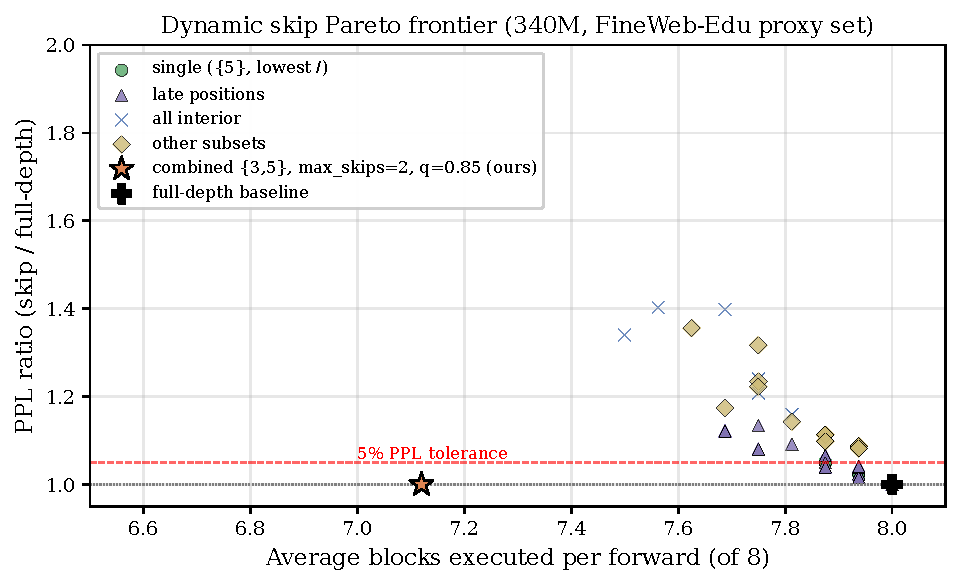
\includegraphics[width=\textwidth]{reskip_pareto.pdf}
\caption{Accuracy--compute Pareto. $\mathcal{P}{=}\{3,5\}$ (orange star) sits below the $5\%$ PPL tolerance.}
\end{subfigure}\hfill
\begin{subfigure}[b]{0.42\textwidth}\centering
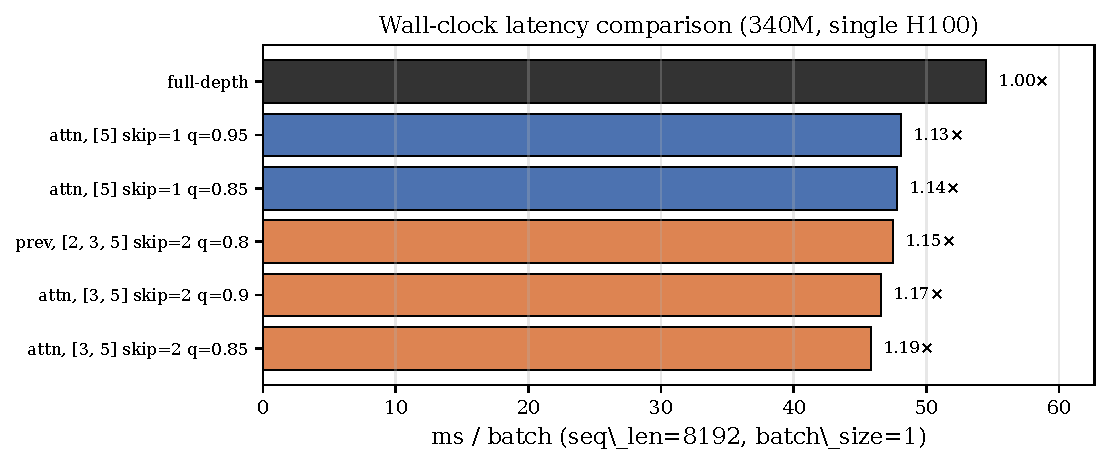
\includegraphics[width=\textwidth]{reskip_latency.pdf}
\caption{Wall-clock at seq $8192$. $\{3,5\}/M{=}2/q{=}0.85$ reaches $1.19\times$.}
\end{subfigure}
\caption{\reskip{} on 340M FineWeb-Edu: position-calibrated dynamic skip with $\mathcal{P}{=}\{3,5\}$ strictly dominates the single-position baseline at zero benchmark drop.}
\label{fig:reskip_pareto_latency}
\end{figure}

%----------------------------------------------------------------------
\section{Retrofit Pareto and breakdowns}
\label{app:retrofit_extras}
%----------------------------------------------------------------------

\subsection{LoRA baselines}
\label{app:lora_baselines}
These auxiliary controls ask whether adding a similar number of trainable parameters through a standard adaptation path is enough to reproduce the text gains. They are pilot controls on an earlier $50/50$ UltraChat $+$ LLaVA mix, not a final-mixture baseline for Tab.~\ref{tab:retrofit_main}. LoRA $r{=}32$ on $q,v$: LAMBADA acc $0.540$ / $0.516$ (two seeds), HellaSwag $0.510$ / $0.524$. LoRA $r{=}16$ on $q,k,v,o$: LAMBADA $0.534$, HellaSwag $0.492$. LoRA $r{=}8$ on MLP: LAMBADA $0.514$, HellaSwag $0.510$. Mean LAMBADA across the four runs is $0.526$, $-0.6$pp below base ($0.532$) and $-5.0$pp below the matched $\gamma{\to}1$ retrofit on that mix ($0.576$). Mean HellaSwag $0.509$ is $+0.3$pp over base versus retrofit's $+1.6$pp. These controls rule out a simple parameter-count-only explanation under a related SFT setting, but they do not prove that all quality gains come uniquely from routing.

\subsection{\texorpdfstring{Static-pruning baseline at the VLM scale (Gromov drop-$k$)}{Static-pruning baseline at the VLM scale (Gromov drop-k)}}
\label{app:gromov_pruning}
The $340$M decision-rule ablation (Tab.~\ref{tab:b1b2_decision_rule})
shows that \emph{single-position} static skip and random skip both
degrade on language tasks. The complementary question at the VLM
scale is whether \emph{full-layer} static pruning---the standard
``remove the least useful blocks'' baseline used by
\citet{gromov2024unreasonable}---can match the accuracy floor that the
retrofit operates above. We rank the $28$ Qwen$3$-VL-$2$B layers by
the Gromov angular-distance criterion (computed on a
FineWeb-Edu calibration set with the LM-head only; no fine-tuning),
remove the $k$ lowest-distance layers, and re-evaluate on
\texttt{lmms-eval}. Tab.~\ref{tab:gromov_pruning_2b} reports drop-$4$
(layers $\{23,24,25,26\}$) and drop-$8$ (additionally
$\{12,13,14,22\}$).

\begin{table}[h]
\caption{\textbf{Static layer pruning on Qwen$3$-VL-$2$B} (Gromov-style angular-distance ranking, no retraining), \texttt{lmms-eval} full splits. Companion to the $340$M in-block decision-rule ablation in Tab.~\ref{tab:b1b2_decision_rule}: spans the \emph{full-layer} vs.\ \emph{single-position-within-block} skip dimension. Pruning $4$ of $28$ layers ($14\%$) costs $-16$pp AI2D, $-6$pp MMMU, $-5$pp MMStar, $-65$pp OCRBench; pruning $8$ ($29\%$) sharply degrades every cell. The retrofit (Tab.~\ref{tab:retrofit_main}) operates at $0$ removed layers, $0$pp loss, and additionally lifts the base; \reskip{} on the retrofit at $q{=}0.85$ holds within $1$pp on LAMBADA (Tab.~\ref{tab:retrofit_pareto}).}
\label{tab:gromov_pruning_2b}
\centering\small
\setlength{\tabcolsep}{4pt}
\begin{tabular}{lccccc}
\toprule
Configuration & AI2D & MMMU & MMStar & OCRBench & RWQA \\
\midrule
Qwen3-VL-2B (base, $L_{\text{rm}}{=}0$)            & $0.736$ & $0.414$ & $0.536$ & $0.772$ & $0.648$ \\
Gromov drop-$4$ (layers $\{23,24,25,26\}$)         & $0.5732$ & $0.3556$ & $0.4906$ & $0.1240$ & $0.3791$ \\
Gromov drop-$8$ (drop-$4$ $\cup$ $\{12,13,14,22\}$) & $0.0683$ & $0.2389$ & $0.0190$ & $0.0030$ & $0.1451$ \\
\midrule
$+$ \retrofit{} v3 ($L{=}4$, $10$k; Tab.~\ref{tab:retrofit_main}) & $\mathbf{0.758}$ & $\mathbf{0.432}$ & $\mathbf{0.536}$ & $\mathbf{0.814}$ & $\mathbf{0.661}$ \\
\bottomrule
\end{tabular}
\end{table}

The pattern matches the in-block $340$M observation: any
\emph{unconditional} block removal (single-position static at
$340$M, full-layer Gromov at $2$B) destroys benchmark accuracy at
the VLM scale even at modest pruning fractions, while
input-dependent skip on top of an \attnres{} routing structure
preserves it. We do not attempt to retrain the pruned model; the
intent is a free static-baseline floor for the cost-quality
trade-off, not a tuned competitor.\footnote{Pruned cells additionally
exhibit POPE generation drift below the strict yes/no surface
(drop-$4$ pope-acc $0.021$, drop-$8$ $0.500$ via accidental
all-``yes'' decoding), so we drop POPE from the table.}

\subsection{\reskip{} on the canonical retrofit: text Pareto and cross-modality consistency}
\label{app:retrofit_pareto}
On the canonical $L{=}4$ v3 $10$k retrofit, applied to LAMBADA-$500$ as the language-modality cross-check of the LIBERO Pareto (Tab.~\ref{tab:vla_reskip_pareto}), \reskip{} produces the same shape as on action: lossless at the conservative end, collapsing once $q$ moves below the action distribution's mean. Same $\mathcal{P}{=}\{1,4\}$, $M_{\max}{=}2$ as the $2$B VLA cell.

\begin{table}[h]
\caption{\textbf{Cross-modality \reskip{} consistency.} LAMBADA-$500$ on the canonical $L{=}4$ v3 retrofit, $\mathcal{P}{=}\{1,4\}, M{=}2$, $\tau$ calibrated on $32$ held-out LAMBADA prefixes at quantile $q$. Same operating-point structure as the LIBERO 4-suite Pareto: near-lossless above the calibration distribution mean ($q{\geq}0.85$); sharp degradation below, where the threshold instructs the router to skip blocks it is normally executing.}
\label{tab:retrofit_pareto}
\centering\small
\begin{tabular}{ccccc}
\toprule
$q$ & LAMBADA acc & LAMBADA ppl & $\Delta$ acc vs no-skip & avg.\ skips / forward \\
\midrule
no-skip ($M{=}0$) & $0.5700$ & $4.526$ & --- & $0.00$ / $\le 7$ \\
$0.85$ & $0.5600$ & $5.258$ & $-1.0$ & $0.19$ / $2$ \\
$0.50$ & $0.4120$ & $12.550$ & $-15.8$ & $1.06$ / $2$ \\
$0.30$ & $0.3900$ & $14.005$ & $-18.0$ & $1.17$ / $2$ \\
\bottomrule
\end{tabular}
\end{table}

\subsection{\texorpdfstring{Wall-clock latency: full table including earlier $L{=}2$ and VLA in-backbone}{Wall-clock latency: full table including earlier L=2 and VLA in-backbone}}
\label{app:latency}
Tab.~\ref{tab:retrofit_latency} in the main body reports the canonical $L{=}4$ result. Tab.~\ref{tab:retrofit_latency_full} below shows the full set: the earlier $L{=}2$ partition ($14$ blocks at $2$B) carries a $1.39\times$ structural cost over stock Qwen3-VL-2B because each token pays $14$ router calls, the VLA in-backbone forward (the same retrofit run inside the OFT trainer's backbone forward, \S\ref{sec:vla}) tracks the VLM retrofit within $1\%$ at both partitions, and \texttt{torch.compile} closes the $L{=}2$ residual to $1.16\times$ but is more dramatic on $L{=}4$ where the router count is halved. This table is the basis for the canonical-partition switch from $L{=}2$ to $L{=}4$.

\begin{table}[h]
\caption{\textbf{Forward-pass latency, full sweep} on $1{\times}$H100, bf16, batch $1$, median of $20$ runs after $5$ warmup. Eager rows: stock-HF base vs.\ retrofit at the indicated $L$. Compile rows wrap both with \texttt{torch.compile}, \texttt{dynamic=False}; \texttt{reduce-overhead} captures CUDA graphs, \texttt{max-autotune} additionally tunes per-kernel matmuls. The VLA in-backbone row is the canonical $L{=}4$ retrofit loaded into the OFT trainer's backbone forward (a separate code path) — within $1\%$ of the VLM retrofit cell, confirming the per-block router stack, not the VLA harness, is the structural cost. \emph{Bold:} the canonical operating point of the paper.}
\label{tab:retrofit_latency_full}
\centering\small
\setlength{\tabcolsep}{4pt}
\begin{tabular}{lccccc}
\toprule
Configuration & seq & mode & base (ms) & retrofit (ms) & retrofit / base \\
\midrule
(1) $L{=}2$ retrofit (earlier)       & $1024$ & eager & $15.42$ & $21.25$ & $1.378\times$ \\
(2) $L{=}2$ retrofit (earlier)       & $2048$ & eager & $26.03$ & $36.14$ & $1.388\times$ \\
(3) $L{=}4$ retrofit (canonical)     & $1024$ & eager & $14.91$ & $16.66$ & $1.117\times$ \\
(4) $L{=}4$ retrofit (canonical)     & $2048$ & eager & $25.49$ & $28.53$ & $1.119\times$ \\
\midrule
(5) $L{=}2$ retrofit                 & $1024$ & \texttt{reduce-overhead}  & $9.31$  & $10.78$ & $1.158\times$ \\
(6) $L{=}2$ retrofit                 & $2048$ & \texttt{reduce-overhead}  & $21.25$ & $24.45$ & $1.151\times$ \\
(7) $L{=}4$ retrofit                 & $2048$ & \texttt{reduce-overhead}  & $21.31$ & $22.50$ & $1.056\times$ \\
\textbf{(8) $L{=}4$ retrofit}        & $\mathbf{2048}$ & \textbf{\texttt{max-autotune}} & $\mathbf{21.81}$ & $\mathbf{22.43}$ & $\mathbf{1.029\times}$ \\
\midrule
(9) VLA in-backbone $L{=}4$ retrofit & $2048$ & eager & $25.49$ & $28.79$ & $1.130\times$ \\
\bottomrule
\end{tabular}
\end{table}

The structural per-block router stack (\texttt{stack}$\to$\texttt{RMSNorm}$\to$\texttt{softmax}$\to$\texttt{einsum} over $N$ completed blocks) is small but visible in eager inference. Adapter rank ablation (Appendix~\ref{app:rank_ablation}) confirms the adapter is not the bottleneck ($\leq 2\%$). \texttt{torch.compile} (rows 5--8) collapses the small router gemms into a captured graph and tunes the matmul kernels for retrofit's small shapes, removing most of the $L{=}4$ structural gap. The remaining $2.9\%$ is the cost of the installed routing path at the canonical operating point; fusing the router and skip decision into a single production kernel is an implementation direction rather than a change to the method.

\subsection{Compile vs.\ eager: accuracy parity}
\label{app:compile_accuracy}

The compiled-overhead result of \S\ref{sec:exp_retrofit} requires that \texttt{torch.compile} preserve the retrofit's accuracy. We verified two parity tests on the canonical $L{=}4$ v3 $10$k retrofit.

\paragraph{LAMBADA-$500$ accuracy parity.} Running LAMBADA-$500$ with the retrofit wrapped in \texttt{torch.compile} using default mode and dynamic shapes: acc $0.5720$ compiled vs.\ $0.5700$ eager ($\Delta{=}+0.20$pp), ppl $4.534$ vs.\ $4.526$. Per-target argmax agreement against eager: $98.60\%$ — the residual $1.4\%$ are tokens where eager and compiled both fall within bf16 SDPA jitter and the rank-$1$/rank-$2$ logits flip.

\paragraph{Per-token logit parity.} On real prompt tokens with \texttt{mode="reduce-overhead"} (the inference-time mode used for the speed table): per-token argmax agreement $98.51\%$, max $|\Delta\text{logits}|=0.50$, RMSE $0.060$ — same magnitude as the cache-on/cache-off SDPA jitter on the stock base (Appendix~\ref{app:kv_equiv}). Compile preserves the retrofit's forward to within bf16 evaluation noise; the $1.029\times$ \texttt{base\_compiled} number is at matched accuracy.

\subsection{Block partition sweep}
\label{app:block_partition}
\begin{table}[h]
\caption{Block partition sweep (v3 recipe, $r{=}256$, $\gamma$-curriculum). $L$ is layers-per-block, $N{=}L_{\text{total}}/L$. Per-layer $L{=}1$ underperforms by $2$--$9$pp; the plateau $L\in\{2,4,7\}$ on $2$B reproduces \citet{chen2026attnres}'s $S\in\{2,4,8\}$. We recommend $L{=}4$ on both scales because it preserves quality while reducing router calls.}
\label{tab:block_partition}
\centering\small
\setlength{\tabcolsep}{3pt}
\begin{tabular}{lccccccccccc}
\toprule
Scale & $L$ & $N$ & LAMBADA & $\Delta$L & HellaSwag & MMBench & MMMU & MMStar & AI2D & OCRBench & RWQA \\
\midrule
2B base       & --- & ---  & 0.532  & ---     & 0.506 & 75.77 & 0.414 & 0.536 & 0.736 & 0.772 & 0.648 \\
2B retrofit   & $1$ & $28$ & 0.5645 & $+3.3$  & 0.490 & 76.20 & 0.388 & 0.499 & 0.743 & 0.809 & 0.652 \\
2B retrofit   & $2$ & $14$ & 0.5755 & $+4.4$  & 0.494 & 77.23 & 0.426 & 0.532 & 0.748 & 0.803 & 0.663 \\
\textbf{2B (rec.)} & $\mathbf{4}$ & $\mathbf{7}$  & $\mathbf{0.5650}$ & $\mathbf{+3.3}$  & $\mathbf{0.500}$ & \textbf{78.87} & \textbf{0.432} & \textbf{0.536} & \textbf{0.758} & \textbf{0.814} & 0.661 \\
2B retrofit   & $7$ & $4$  & 0.5155 & $-1.7$  & 0.492 & 77.49 & 0.427 & 0.530 & 0.756 & 0.808 & 0.656 \\
\midrule
4B base       & --- & ---  & 0.576  & ---     & 0.562 & 83.33 & 0.490 & 0.624 & 0.819 & 0.819 & 0.715 \\
4B retrofit   & $1$ & $36$ & 0.5575 & $-1.9$  & 0.523 & 83.33 & 0.497 & 0.538 & 0.783 & 0.768 & 0.694 \\
4B retrofit   & $2$ & $18$ & --     & --      & --    & 84.28 & 0.523 & 0.587 & 0.816 & 0.813 & 0.708 \\
\textbf{4B (rec.)} & $\mathbf{4}$ & $\mathbf{9}$ & $\mathbf{0.6625}$ & $\mathbf{+8.7}$ & $\mathbf{0.552}$ & \textbf{85.22} & 0.521 & \textbf{0.632} & \textbf{0.825} & \textbf{0.824} & \textbf{0.718} \\
4B retrofit   & $6$ & $6$  & 0.6540 & $+7.8$  & 0.554 & 84.79 & \textbf{0.531} & 0.623 & 0.817 & 0.824 & 0.715 \\
\bottomrule
\end{tabular}
\end{table}

\subsection{MMStar subcategory breakdown}
\label{app:mmstar_subcat}
\begin{table}[h]
\caption{MMStar subcategory breakdown for the v3 retrofit. The math, logical, and sci\&tech triple is the ``reasoning over images'' cell where the retrofit shows the largest gain ($+7.9$pp math on $2$B; $+3.9$pp on $4$B). Perception cells (coarse / fine / instance) are at parity or a small regression, consistent with a router that lifts deliberate-reasoning paths rather than altering early perception.}
\label{tab:mmstar_subcat}
\centering\small
\setlength{\tabcolsep}{4pt}
\begin{tabular}{lcccccc}
\toprule
Configuration & math & logical & sci\&tech & coarse & fine & instance \\
\midrule
Qwen3-VL-2B (base)                       & 0.413 & 0.429 & 0.408 & 0.714 & 0.520 & 0.710 \\
$+$ \retrofit{} v3 ($2$B, $L{=}4$)       & \textbf{0.492} & \textbf{0.432} & 0.353 & 0.734 & 0.505 & 0.683 \\
$\Delta$ vs.\ $2$B base                   & $\mathbf{+7.9}$ & $+0.3$ & $-5.5$ & $+2.0$ & $-1.5$ & $-2.7$ \\
\midrule
Qwen3-VL-4B (base)                       & 0.549 & 0.626 & 0.465 & 0.788 & 0.611 & 0.705 \\
$+$ \retrofit{} v3 ($4$B, $L{=}4$)       & \textbf{0.588} & 0.602 & \textbf{0.467} & 0.812 & 0.606 & 0.714 \\
$\Delta$ vs.\ $4$B base                   & $\mathbf{+3.9}$ & $-2.4$ & $+0.2$ & $+2.4$ & $-0.5$ & $+0.9$ \\
\bottomrule
\end{tabular}
\end{table}

%----------------------------------------------------------------------
\section{VLA appendix}
\label{app:vla_section}
%----------------------------------------------------------------------

\subsection{VLA seed variance on 2B}
\label{app:vla_variance}
We ran two seeds for the two $2$B suites where Path 0 / Path B are within evaluation noise on a single seed; \texttt{libero\_spatial} and \texttt{libero\_object} are single runs.
\begin{table}[h]
\caption{Per-seed Qwen3-VL-2B numbers. Seed 1 is the initial run; seed 2 is a fresh environment-reseeded rollout of the same trained checkpoint. The last column shows the values used in Table~\ref{tab:vla_libero}.}
\label{tab:vla_seed_variance}
\centering\small
\begin{tabular}{llccc}
\toprule
Suite & Policy & Seed 1 & Seed 2 & Used in Tab.~\ref{tab:vla_libero} \\
\midrule
\texttt{libero\_goal} & Path 0 ($30$k) & $97.6$ & $97.4$ & $97.4$ \\
\texttt{libero\_goal} & Path B ($30$k) & $97.4$ & $98.6$ & $98.6$ \\
\texttt{libero\_10}   & Path 0 ($30$k) & $92.8$ & $91.4$ & $91.4$ \\
\texttt{libero\_10}   & Path B ($30$k) & $92.6$ & $90.6$ & $92.6$ \\
\bottomrule
\end{tabular}
\end{table}
Aggregating both repeated rollouts gives Path 0 $96.05$ and Path B $96.75$ ($\Delta{=}+0.70$pp), while the Table~\ref{tab:vla_libero} operating-point values give $\Delta{=}+1.30$pp. Both summaries preserve the ranking Path B $>$ Path 0. The main text therefore treats LIBERO as supporting transfer evidence rather than as the primary contribution.

\subsection{VLA landscape: open VLAs on standard benchmarks}
\label{app:vla_landscape}
\begin{table}[h]
\caption{Open VLA landscape on standard benchmarks. LIBERO entries are success rates ($\%$) per task suite. Following common practice, $\pi_0$ and Octo-Base LIBERO numbers are taken from OpenVLA-OFT~\citep{kim2025openvlaoft}, which re-ran all three policies under a uniform LIBERO protocol. Our rows use the $30$k Path B numbers from Table~\ref{tab:vla_libero}.}
\label{tab:vla_landscape}
\centering\small
\setlength{\tabcolsep}{4pt}
\begin{tabular}{lccccccc}
\toprule
Model & \#Params & Spatial & Object & Goal & Long-10 & ref. \\
\midrule
Octo-Base    & 93M & 78.9 & 85.7 & 84.6 & 51.1 & \citep{team2024octo, kim2025openvlaoft} \\
OpenVLA      & 7B  & 84.7 & 88.4 & 79.2 & 53.7 & \citep{kim2024openvla, kim2025openvlaoft} \\
TraceVLA     & 7B  & 84.6 & 85.2 & 75.1 & 54.1 & \citep{zheng2024tracevla} \\
SpatialVLA   & 4B  & 88.2 & 89.9 & 78.6 & 55.5 & \citep{qu2025spatialvla} \\
$\pi_0$      & 3B  & \textbf{96.8} & \textbf{98.8} & 95.8 & 85.2 & \citep{black2024pi0, kim2025openvlaoft} \\
\midrule
\rowcolor{black!6}
\textbf{Qwen3-VL-2B + AR-Retrofit + OFT} (\emph{ours}) & 2B & $\mathbf{97.8}$ & $99.6$ & $\mathbf{98.6}$ & $92.6$ & this work \\
\rowcolor{black!6}
\textbf{Qwen3-VL-4B + AR-Retrofit + OFT} (\emph{ours}) & 4B & $94.6$ & $\mathbf{99.8}$ & $\mathbf{98.2}$ & $\mathbf{94.2}$ & this work \\
\bottomrule
\end{tabular}
\end{table}

\subsection{VLA \reskip{} setup: per-block drift and eligible-set selection}
\label{app:vla_pareto}

The \reskip{} eligible set $\mathcal{P}$ for each scale is selected from a per-block ablation \emph{on the trained Path B policy}, not on the VLM retrofit alone, because the VLA action stream activates a different routing distribution than the language stream. We measure per-block action-drift MSE on a $24$-sample sim trajectory: the policy is run with no skip and with each block individually skipped; the per-step action MSE between the skipped and no-skip rollouts is the per-block ``cost of removing this block on the action distribution''. The two safest blocks per scale form $\mathcal{P}$.

\textbf{2B Path B 30k} per-block action-drift MSE (sorted ascending, in units $\times 10^{-3}$):
block~$1$: $0.4$; block~$4$: $34.0$; block~$0$: $58.1$; block~$5$: $87.0$; remaining blocks $>$$100$. Selecting the two lowest: $\mathcal{P}_{2\text{B}}=\{1, 4\}$.

\textbf{4B Path B 30k} per-block action-drift MSE: block~$1$: $0.6$; block~$2$: $11.0$; block~$0$: $34.0$; block~$3$: $63.0$; remaining $>$$120$. Selecting: $\mathcal{P}_{4\text{B}}=\{1, 2\}$.

\paragraph{Per-scale eligibility.} The eligible set is selected separately for each model scale because the action-stream routing distribution and per-block drift are scale dependent. This is the per-scale half of the modality-aware skip protocol: $\alpha$ provides the online signal, while action-drift calibration selects the safe candidate blocks for the policy being deployed.

\paragraph{Threshold calibration.} Per-block thresholds $\tau_n$ are the $q$-th empirical quantile of $w_{\text{recent},n}$ over $31{,}286$ ($2$B) / $31{,}257$ ($4$B) sim-rollout records (one record per decoded action token across many trajectories). The Tab.~\ref{tab:vla_reskip_pareto} numbers use this protocol. A separate ``Method A'' that calibrates on retrofit pretokenized data (as if the VLA were just a long-context LM) lands at a conservative operating point that mimics $q{=}0.99$ on the action distribution; we use it as a sensitivity comparator in our ablations and recommend the action-distribution-calibrated thresholds for any deployment.

\paragraph{Cross-modality threshold calibration.} Language-calibrated thresholds and action-calibrated thresholds correspond to different effective skip rates because the action stream has a different $w_{\text{recent}}$ distribution. We therefore calibrate $\tau_n$ on the action distribution for LIBERO rather than transferring the LAMBADA thresholds unchanged. This is the same calibration principle used in the main method: routing decides when to skip, while the eligible set and thresholds are selected on the deployment distribution.

\subsection{VLA planned follow-ups}
\label{app:vla_future}
\emph{Per-modality, per-token-class \reskip{}.} The Tab.~\ref{tab:vla_reskip_pareto} thresholds are calibrated on the action distribution as a whole; an obvious refinement is per-modality $(\mathcal{P}^{(m)}, \tau_n^{(m)}, M_{\max}^{(m)})$ within a single rollout (vision tokens, language tokens, action tokens). Working hypothesis: vision $\alpha$ concentrates on early blocks, while action $\alpha$ spreads to late blocks and benefits from more conservative late-block skipping. \emph{Fused routing kernels.} A static-graph variant of the skip rule could further reduce the installed-path runtime. \emph{Edge hardware.} Wall-clock is H100 / bf16; RTX 4090 / Jetson Orin direct measurement is planned.

\section{NeurIPS Paper Checklist}
\label{app:checklist}
\begin{enumerate}
\item \textbf{Claims.} Yes. The abstract, introduction, and conclusions state the main claims and separate the retrofit contribution from calibrated skipping, VLA transfer, and systems characterization.
\item \textbf{Limitations.} Yes. Appendix~\ref{app:limitations} lists architecture coverage, hardware scope, block-level routing granularity, and per-modality calibration limits.
\item \textbf{Theory assumptions.} Not applicable. The paper is empirical and algorithmic; all equations define implemented objectives or routing rules.
\item \textbf{Experimental reproducibility.} Yes. Sections~\ref{sec:reskip}--\ref{sec:vla_results} and the appendix specify model scales, block partitions, training steps, datasets, calibration rules, and evaluation protocols.
\item \textbf{Open access to code and data.} Yes. Experiments use public datasets and benchmarks; implementation details and release plan are described under the anonymous submission policy.
\item \textbf{Compute.} Yes. Main text and appendices report GPU type, training steps, rough GPU-minutes / GPU-hours, and latency measurement settings.
\item \textbf{Dataset and benchmark provenance.} Yes. All public datasets and benchmarks are cited; LIBERO and lmms-eval protocols are described with rollout counts or split usage.
\item \textbf{Human subjects.} Not applicable. No new human-subject data are collected.
\item \textbf{Privacy.} Not applicable beyond the privacy considerations of the cited public datasets.
\item \textbf{Licenses.} Yes. Public datasets/models are cited; release artifacts will include license metadata.
\item \textbf{Broader impacts.} Yes. The work targets lower inference cost and adaptive computation in pretrained models; no safety-critical deployment is claimed.
\item \textbf{Safeguards.} Yes. VLA thresholds are calibrated per model and action distribution; cross-modality transfer failures are explicitly documented as a deployment risk.
\end{enumerate}

\end{document}
